\documentclass[aps,prx,preprint,superscriptaddress,nofootinbib]{revtex4-2}

\usepackage{amsmath,amssymb,amsfonts}
\usepackage{graphicx}
\graphicspath{{figures/}}
\usepackage{longtable,booktabs,array}
\usepackage{calc}
\providecommand{\real}[1]{#1}
\usepackage{xcolor}
\usepackage[colorlinks=true,linkcolor=blue,citecolor=blue,urlcolor=blue]{hyperref}

% Arabic section and subsection numbering, matching the textual
% "Section N" / "Section N.M" references used throughout the prose.
\renewcommand{\thesection}{\arabic{section}}
\renewcommand{\thesubsection}{\thesection.\arabic{subsection}}
% Clear REVTeX's subsection label prefix: \p@subsection prepends the section
% number, but \thesubsection above already carries it, so a subsection \ref
% would otherwise render the section number twice.
\makeatletter\renewcommand{\p@subsection}{}\makeatother

% pandoc compatibility
\providecommand{\tightlist}{\setlength{\itemsep}{0pt}\setlength{\parskip}{0pt}}
\providecommand{\passthrough}[1]{#1}

\begin{document}

\title{Two spectral functionals set the exponential cost\\ of shadow moment estimation}

\author{Alexander Messerlian}
\affiliation{Independent Researcher}
\author{Ziwei Gu}
\affiliation{Harvard John A. Paulson School of Engineering and Applied Sciences}

\date{August 6, 2026}

\begin{abstract}
Classical shadows estimate moments \(\mathrm{Tr}(\rho^k)\) from randomized single-copy
measurements. The finite-sample variance of the resulting U-statistic splits into projection terms
of different budget order --- a Hoeffding decomposition \cite{hoeffding1948, serfling1980} stated
for shadows in \cite{huang2020shadows}, with two known decay regimes
\cite{elben2020mixed, aasen2026limitations} --- and the state-dependent variances fixing their
ratio have been bounded rather than evaluated. We evaluate them exactly for an arbitrary state.
The exponential rate of the cost is then not a constant of the protocol but a spectral functional
of the state: \(\zeta_2\) is a Pauli sum with kernel \(14^{-|P|}\), giving
\(7^n - 1 \le \zeta_2 \le (17/2)^n\) for every state and confining the per-qubit base to
\([7, 17/2]\) in the limit, while \(\zeta_1\) is a cubic contraction of the same second-moment
identity. Their ratio is the budget \(M^* = \zeta_2/(2\zeta_1)\) at which the effective error
exponent crosses over, with
\(\mathrm{base}(M^*) = \mathrm{base}(\zeta_2)/\mathrm{base}(\zeta_1)\) exactly. The branches
differ: \(28/5\) for spread spectra, and exactly \(5\) for every pure product state, where
\(\zeta_1 = (3/2)^n - 1\) and \(\zeta_2 = (15/2)^n - 1\) at any orientation --- so purity alone
fixes neither factor. The law holds statewise, not merely on average: across a family whose
thresholds span a decade, predicted and measured per-state error agree with rank correlation
\(0.87\) and slope \(0.97\), against \(0.26\) on a fixed-estimand control too narrow to resolve
an ordering. The threshold is also estimable from the snapshots alone, by unbiased four-block
estimators whose cost grows more slowly in \(n\) than \(M^*\) and falls below it by eight
qubits. Fed into two exact bias laws for collective measurement it becomes a plug-in criterion,
nothing fitted to the crossover data, for when two-copy measurement attains the lower RMSE at
equal copy budget, placing every resolving cell within one qubit across five state families.
Results are simulation to ten qubits; at \(k \ge 3\) the projection variances are numerical.
\end{abstract}


\maketitle

\hypertarget{introduction}{%
\section{Introduction}\label{introduction}}

At the maximally mixed state, estimating purity from classical shadows is as expensive as it ever
gets. That sounds backwards. The estimand is \(2^{-n}\), nearly zero, and every snapshot returns
\(\mathrm{Tr}(G\rho) = 2^{-n}\) deterministically, so the first-order projection variance
\(\zeta_1\) vanishes identically. What does not vanish is the kernel term: the single-qubit second
moment \(\mathbb{E}[\mathrm{Tr}(G_1G_2)^2]\) equals \(7\) for a maximally mixed qubit, so
\(\zeta_2 = 7^n - 4^{-n}\), and the estimator's error is of order \(7^{n/2}/M\) against a target
shrinking as \(2^{-n}\). Low purity does not remove the exponential cost; it concentrates it.

The exponential is therefore a property of the estimator, and the question this paper answers is
what fixes its rate. The answer is not the purity, and not a constant of the protocol. It is two
spectral functionals of the state.

The finite-sample variance of the shadow U-statistic splits into projection terms of different
budget order --- the standard Hoeffding decomposition \cite{hoeffding1948, serfling1980}, stated
for shadows in \cite{huang2020shadows} --- and that the resulting decay rate changes with the
budget is established: Elben et al.~\cite{elben2020mixed} state both regimes and plot them, and
Aasen and G\"arttner \cite{aasen2026limitations} track the exponent migrating between them under
detector noise. What those analyses do not do is evaluate the coefficients. Bounding \(\zeta_1\)
and \(\zeta_2\) separately constrains their ratio not at all, and the exact second moment that
would fix it is applied in the literature to worst-case sample complexity rather than to a state.

\textbf{Thesis.} We evaluate the two projection variances exactly for an arbitrary state at
\(k = 2\), from the second-moment identity of \cite{huang2020shadows}: \(\zeta_2\) as a Pauli sum
with kernel \(14^{-|P|}\), \(\zeta_1\) as a cubic contraction of the same identity. Three things
follow. First, \(7^n - 1 \le \zeta_2 \le (17/2)^n\) for every state, so the per-qubit exponential
base is confined to \([7, 17/2]\) in the limit, and which value a state realizes is set by how its
Pauli weight is distributed rather than by its purity: a Haar-random pure state and a pure product
state, both of purity one, sit at \(7\) and at \(15/2\). Second, the budget at which the effective
error exponent crosses over is \(M^* = \zeta_2/(2\zeta_1)\), and its growth base factorizes as
\(\mathrm{base}(\zeta_2)/\mathrm{base}(\zeta_1)\) exactly, giving \(28/5\) for spread spectra and
exactly \(5\) for every pure product state. Third, because these are statewise functionals they
predict what an individual state does, which we verify by ordering states within a family whose
thresholds span a decade --- and, on a fixed-estimand control, show cannot be verified at all.

That the quantities are exact does not make them usable, since evaluating them needs the state.
We close that gap too, with unbiased estimators of both variances built from four disjoint blocks
of a pilot shadow budget, which never form the Pauli spectrum and whose cost grows more slowly in
\(n\) than the threshold they locate.

Set against two exact bias laws for collective measurement, the same machinery yields a plug-in
criterion, with nothing fitted to the crossover data, for the size at which a two-copy measurement
attains the lower RMSE at equal copy budget. That application is where the practical stakes sit,
and they are not small: on the noisy-pure states we benchmark, at a fixed budget and ten qubits,
the single-copy purity estimate projected into the interval purity is known a priori to occupy has
RMSE \(0.582\), while a constant fixed at the midpoint of that interval, which never looks at the
data, has \(0.310\). From seven qubits on, the single-copy route is worse than that constant.
Before projection the estimator is still unbiased; it is the spread that has become useless.

That matters because the quantity is not exotic. The moments \(\mathrm{Tr}(\rho^k)\) are the entry
point to much of what one wants to know about an unknown state: the second is the purity, their
logarithms give the R\'enyi entropies, moments of the partial transpose furnish PPT entanglement
criteria and bounds on negativity, and purity enters error-mitigation protocols such as virtual
distillation. Any experiment characterizing the state its device actually prepared needs these
numbers.

We compare two routes throughout. The single-copy route measures one copy at a time in randomized
local bases, building classical shadows \cite{huang2020shadows}, and forms an unbiased U-statistic
from the snapshots; it uses no entangling gates. The collective route holds \(k\) copies
simultaneously and measures the cyclic-permutation operator, whose expectation is exactly
\(\mathrm{Tr}(\rho^k)\); it has \(O(1)\) variance but requires entangling operations across
copies. The asymptotic separation between them is settled. Single-copy strategies require
exponentially more samples than collective ones for a family of learning tasks
\cite{huang2022advantage,chen2022separations}, and for protocols restricted to an identical
single-copy projection-valued measurement the lower bound for purity estimation is
\(\Omega(\max\{1/\varepsilon^2, 2^{n/2}/\varepsilon\})\) \cite{gong2024purity}. What is not settled
is the question an experimentalist faces: at this noise level and this system size, which route
has the lower RMSE at equal state-copy budget?

The gap is visible in recent work. A May 2026 study of quantum machine learning advantage on tens
of noisy qubits \cite{qmladvantage2026} declined to give its measure-first protocol multi-copy
access, citing both a result specific to its learning task and the resource demands of multi-copy
entangled measurements. That task is not moment estimation, but the caution about resource cost is
a premise we can test quantitatively. On the theory side, \cite{noisylearning2026} shows that the
exponential two-copy advantage for purity \emph{testing} collapses under local depolarizing noise;
their task is testing and ours is estimation, a distinction we take up in Section 8. The caution
is reasonable. What has not been available is a prediction of the size at which it stops applying.

\begin{center}\rule{0.5\linewidth}{0.5pt}\end{center}

\hypertarget{setting-and-estimators}{%
\section{Setting and estimators}\label{setting-and-estimators}}

\hypertarget{local-random-unitary-classical-shadows}{%
\subsection{Local random-unitary classical
shadows}\label{local-random-unitary-classical-shadows}}

Let \(\rho\) be an unknown \(n\)-qubit state. A single snapshot is
produced by drawing an independent Haar-random single-qubit unitary
\(U_q\) for each qubit, applying \(\bigotimes_q U_q\), measuring in the
computational basis to obtain a bitstring \(b\), and forming

\[G = \bigotimes_{q=1}^{n} \left( 3\, U_q^\dagger \lvert b_q \rangle \langle b_q \rvert U_q - \mathbb{I} \right).\]

The snapshot is an unbiased estimator of the state,
\(\mathbb{E}[G] = \rho\). A budget of \(M\) snapshots consumes \(M\)
copies of \(\rho\).

\hypertarget{the-estimator-must-be-the-exact-u-statistic}{%
\subsection{The estimator must be the exact
U-statistic}\label{the-estimator-must-be-the-exact-u-statistic}}

The \(k\)-th moment is estimated by the U-statistic over distinct
\(k\)-tuples of snapshots,

\[U_M = \binom{M}{k}^{-1} \sum_{i_1 < \cdots < i_k} h(G_{i_1}, \ldots, G_{i_k}), \qquad h(g_1, \ldots, g_k) = \frac{1}{k!} \sum_{\pi \in S_k} \mathrm{Re}\,\mathrm{Tr}\!\left( g_{\pi(1)} \cdots g_{\pi(k)} \right),\]

which is exactly unbiased: \(\mathbb{E}[U_M] = \mathrm{Tr}(\rho^k)\).

The tuples are formed exhaustively rather than sampled. Forming them from
already-collected snapshots is classical post-processing and consumes no
additional copies, so subsampling saves nothing physical while inflating
the variance: in our sweeps it inflated the single-copy RMSE by a
factor of about five at \(n = 2\) and more than fiftyfold at \(n = 4\),
enough to reverse the benchmark's conclusion. Any
single-copy-versus-collective comparison must use the exact estimator on
the single-copy side.

For \(k = 2\) the full U-statistic has an exact closed form, and the two
ways of evaluating it trade \(M\) against \(n\). The power-sum reduction
\(\mathrm{Tr}(S^2) - \sum_i \mathrm{Tr}(G_i^2)\), with \(S = \sum_i G_i\),
is linear in \(M\) but builds dense \(2^n \times 2^n\) matrices at
\(O(M 4^n)\); we instead use
the per-qubit factorization
\(\mathrm{Tr}(G_i G_j) = \prod_q \mathrm{Tr}(G_i^q G_j^q)\), forming an
\(M \times M\) pairwise-trace matrix in \(O(M^2 n)\) time. For \(k = 4\)
no complete power-sum reduction exists, because the snapshots do not
commute; Appendix A gives an exact construction by M\"obius inversion over
the 15 set partitions of the four cyclic slots, with the alternating
partition evaluated by tensor contraction, matching brute-force
enumeration to \(\lesssim 10^{-13}\).

\hypertarget{the-collective-route}{%
\subsection{The collective route}\label{the-collective-route}}

Let \(C_k\) be the cyclic permutation operator on \(k\) registers of
dimension \(d = 2^n\). It satisfies

\[\mathrm{Tr}\!\left( C_k\, \rho^{\otimes k} \right) = \mathrm{Tr}(\rho^k), \qquad \mathrm{Tr}(C_k) = d,\]

the second identity because the cyclic permutation has a single cycle, and
it is what makes the depolarizing bias law of Section 6.1 come out linear
in the noise rate.

We use the destructive SWAP test rather than the ancilla-based
controlled-SWAP construction, which decomposes into many two-qubit gates
and would be dominated by gate noise on current hardware. Two copies are
prepared on \(2n\) qubits; for each pair \((i, i+n)\) a CNOT is applied
with control \(i\) and target \(i+n\), followed by a Hadamard on qubit
\(i\), and all \(2n\) qubits are measured. The purity is recovered by the
parity rule

\[\mathrm{Tr}(\rho^2) = \sum_{\text{bitstrings}} (-1)^{\,\#\{\,i \,:\, a_i = b_i = 1\,\}} \, P(\text{bitstring}),\]

where \(a_i, b_i\) are the outcomes on the two copies of qubit \(i\). The
circuit uses exactly \(n\) two-qubit gates, requires no ancilla, and has
depth two after state preparation; we verified the sign rule against exact
simulation to \(10^{-16}\) (Appendix B). That gate count is what makes the
measurement overhead of the collective route two two-qubit gates, a compilation
fact we return to in Section 2.6.

This construction is specific to \(k = 2\), where \(C_2\) is Hermitian
with eigenvalues \(\pm 1\) so its expectation is directly a two-valued
measurement. For \(k \geq 3\) the cyclic operator is not Hermitian and no
analogous destructive parity test exists, so we take the standard
ancilla-based Hadamard test: an ancilla in \(|+\rangle\), a
controlled-\(C_k\) on the \(k\) copies, and an \(X\)-basis measurement of
the ancilla, whose \(\pm 1\) outcome has expectation
\(\mathrm{Re}\,\mathrm{Tr}(C_k \rho^{\otimes k}) = \mathrm{Tr}(\rho^k)\).
Its shot variance is \(1 - \mu^2\) exactly as at \(k = 2\), which is the
model used for all \(k\) in Section 7. The cost is not comparable:
transpiled to a published square-lattice coupling map, the controlled cyclic shift on
\(kn\) qubits uses about ten times the two-qubit gate count of the
\(k = 2\) destructive test at \(k = 3\) and about sixteen at \(k = 4\),
and needs an ancilla and routing it does not. Our \(k \geq 3\) results are
simulated, and the gate counts of Section 2.6 are for \(k = 2\) only.

\hypertarget{copy-fair-accounting}{%
\subsection{Copy-fair accounting}\label{copy-fair-accounting}}

A single-copy protocol at budget \(M\) consumes \(M\) copies of
\(\rho\). A \(k\)-copy collective test at budget \(M\) consumes \(\lfloor M/k \rfloor\)
measurements, each using \(k\) copies (the swept budgets are not all multiples of \(k\)). All comparisons in this paper
hold the total number of state copies fixed.

\hypertarget{the-state-ensemble-is-not-a-free-choice}{%
\subsection{The state ensemble is not a free
choice}\label{the-state-ensemble-is-not-a-free-choice}}

The variance of shadow-based purity estimation scales with the purity of
the state being measured, a fact we derive exactly in Section 3.3. The
consequence is a trap, though not the one it first appears to be. A random
Ginibre state under heavy depolarizing noise has purity approaching
\(2^{-n}\), and a quantity that is approximately zero is easy to estimate
at fixed absolute error, though not at fixed relative precision, nor
for testing, where the gap to be resolved shrinks too (Section 8). What
does not follow is that the estimator is well behaved there.

Low purity does not remove the exponential cost; it concentrates it. At
\(\rho = \mathbb{I}/2^n\) every snapshot gives
\(\mathrm{Tr}(G\rho) = 2^{-n}\) deterministically, so \(\zeta_1 = 0\)
exactly and \(M^* = \zeta_2/(2\zeta_1)\) diverges, putting the estimator
in the higher-order regime at every budget. The kernel term does not
vanish with it: the single-qubit second moment
\(\mathbb{E}[\mathrm{Tr}(G_1 G_2)^2]\) is \(7\) for a maximally mixed
qubit, so \(\zeta_2 = 7^n - 4^{-n}\), and the variance
\(2\zeta_2 / M(M-1)\) gives an error of order \(7^{n/2}/M\),
exponential in \(n\), against a target itself shrinking as \(2^{-n}\).

The exponential is therefore a property of the estimator, not of
high-purity states. Its leading exponential rate is set by
\(\zeta_2\): purity alone does not fix it, and what does is how the
state's Pauli weight is distributed. That rate is \(7\) per qubit at the
maximally mixed state and for the spread-spectrum ensembles evaluated
here, and larger for stabilizer-structured spectra
(Section~\ref{sec:zeta-closed-form}). Purity governs \(\zeta_1\), and so
\(M^*\) and the exponent, not the exponential itself. The ensemble
nonetheless decides what the benchmark measures: at
\(\rho = \mathbb{I}/2^n\) the collective bias also vanishes identically
for every \emph{unital} channel, since \(\mathrm{Tr}(\rho^k)\) then sits
exactly on the depolarizing floor \(2^{n(1-k)}\), so both routes
degenerate at once and the comparison stops being informative. The
restriction matters: amplitude damping is not unital, and carries
\(\mathbb{I}/2\) to a state of purity \((1 + \gamma^2)/2\).

We therefore benchmark on noisy-pure states, a prepared pure state under
modest depolarizing noise,

\[\rho = (1-q)\lvert \psi \rangle \langle \psi \rvert + q\,\mathbb{I}/2^n, \qquad \lvert \psi \rangle \sim \text{Haar}, \qquad q \in [0.05,\, 0.3],\]

whose purity is stable across the sizes tested but set by \(q\),
approaching \((1-q)^2\) at large \(n\): about \(0.90\) at \(q = 0.05\),
\(0.81\) at the representative \(q = 0.1\), and \(0.49\) at \(q = 0.3\).
These states keep the problem hard and meaningful at once: the moment
is of order one, so an absolute error is a statement about something, and
the collective route has a bias to pay, so the routes are in competition.
Choosing the wrong ensemble does not make the estimator cheap; it makes
the comparison vacuous.

\hypertarget{what-the-collective-circuit-costs-to-compile}{%
\subsection{What the collective circuit costs to compile}\label{sec:compilation}}

The collective route's overhead is often quoted as the reason not to use it, so it is worth
separating what is a compilation fact from what is a device measurement. The counts below are the
former: they are what a transpiler returns for a stated circuit against a published coupling map,
and they need no device access to reproduce.

For \(k = 2\) the destructive test adds \(n\) two-qubit gates and depth two on top of state
preparation, with no ancilla. Transpiled onto a published square-lattice map with a native
\(\{\mathrm{CZ}, R_x, R_z\}\) basis, the \(n = 2\) Bell instance uses four CZ gates --- two to
prepare each copy and two for the pairing --- with zero routing overhead, and the GHZ ladders at
\(n = 3, 4\) map with zero routing at \(3n - 2\) CZ gates and nest inside one another. Structured
states on a matched topology are therefore cheap to pair; generic states are not, and how much
they cost depends on the state-preparation synthesis, so we make no claim there.

For \(k \ge 3\) the ancilla-based Hadamard test is the relevant circuit and it is not comparable.
Transpiled to the same map, the controlled cyclic shift on \(kn\) qubits uses about ten times the
two-qubit gate count of the \(k = 2\) destructive test at \(k = 3\) and about sixteen times at
\(k = 4\), and needs an ancilla and routing the destructive test does not. Every \(k \ge 3\) result
in this paper is a simulation of an idealized bounded-outcome primitive that carries none of that
cost, and the reader should read those sizes as an upper bound on what the collective route buys.

These are gate counts, not error budgets. What they establish is that the entangling overhead is
not the binding constraint for the structured \(k = 2\) circuits we study; what binds instead is
the statistical failure of the single-copy estimator, which Section~\ref{where-single-copy-estimation-stops-being-useful}
quantifies. A companion study takes up how the collective route behaves on a real device, where
neither gate counts nor an idealized primitive are the whole story.

\begin{center}\rule{0.5\linewidth}{0.5pt}\end{center}

\hypertarget{the-single-copy-variance-law}{%
\section{The projection variances}\label{the-single-copy-variance-law}}

\hypertarget{the-hoeffding-decomposition-gives-the-variance-exactly}{%
\subsection{The Hoeffding decomposition gives the variance
exactly}\label{the-hoeffding-decomposition-gives-the-variance-exactly}}

For a symmetric kernel \(h\) of order \(k\), define the \(c\)-th order
projection and its variance,

\[h_c(g_1, \ldots, g_c) = \mathbb{E}_{G_{c+1}, \ldots, G_k}\!\left[ h(g_1, \ldots, g_c, G_{c+1}, \ldots, G_k) \right], \qquad \zeta_c = \mathrm{Var}\!\left[ h_c(G_1, \ldots, G_c) \right].\]

The variance of the U-statistic is then exactly

\[\boxed{\;\mathrm{Var}(U_M) = \binom{M}{k}^{-1} \sum_{c=1}^{k} \binom{k}{c} \binom{M-k}{\,k-c\,} \zeta_c \;}\]

the standard Hoeffding decomposition \cite{hoeffding1948, serfling1980},
for which we claim no novelty; what is new is the closed-form evaluation
of the second-order \(\zeta_c\) and the threshold their ratio fixes
(Section~\ref{sec:zeta-closed-form}). For \(k = 2\) it reduces to

\[\mathrm{Var}(U_M) = \frac{4(M-2)\,\zeta_1 + 2\,\zeta_2}{M(M-1)}, \qquad \zeta_1 = \mathrm{Var}\!\left[\mathrm{Tr}(G\rho)\right], \quad \zeta_2 = \mathrm{Var}\!\left[\mathrm{Tr}(G_i G_j)\right].\]

We verified the general formula against brute-force Monte Carlo of the
exact estimator at \(k = 3\) and \(k = 4\), on noisy-pure, GHZ, and
low-rank states, with all ratios within 3\%, and confirmed it reduces to
the \(k=2\) form at a ratio of \(1.000000\). The law is exact, not
asymptotic, at every budget.

Because the kernel is multilinear in the snapshots, every projection
variance depends on the shadow ensemble only through its second-moment
matrix, and local Haar single-qubit shadows and local Pauli-basis shadows
have identical second-moment matrices, so all results of this section hold
for either. One subtlety is easy to miss: for \(k = 2\) the second-order
projection \emph{is} the kernel, so \(\zeta_2\) is the kernel variance,
but for \(k \geq 3\) it is not: \(\zeta_2\) is the two-argument
projection and the kernel variance is \(\zeta_k\). Substituting one for
the other is wrong by roughly a factor of seven and corrupts any
higher-moment variance estimate while appearing to work at \(k = 2\).

\hypertarget{two-terms-compete-and-their-ratio-is-a-budget-threshold}{%
\subsection{Two terms compete, and their ratio is a budget
threshold}\label{two-terms-compete-and-their-ratio-is-a-budget-threshold}}

The exact variance contains two competing terms. At large \(M\) the linear
term dominates,

\[\mathrm{Var}(U_M) \approx \frac{4\zeta_1}{M} \quad \Longrightarrow \quad \mathrm{RMSE} \propto M^{-1/2}, \qquad \alpha = \tfrac{1}{2},\]

the familiar statistical scaling a fixed-exponent bound predicts; at small
\(M\) the higher-order term dominates,

\[\mathrm{Var}(U_M) \approx \frac{2\zeta_2}{M^2} \quad \Longrightarrow \quad \mathrm{RMSE} \propto M^{-1}, \qquad \alpha = 1.\]

and the two are equal at

\[\boxed{\;M^* = \frac{\zeta_2}{2\zeta_1}\;}\]

the balance point of the two large-\(M\) forms. The exact numerator terms
balance at a point differing from this by an additive constant, immaterial
once \(M^*\) is large, and nothing that follows depends on the choice
because the predicted exponents are computed from the exact variance
formula rather than from \(M^*\). Which side of \(M^*\) an experiment sits
on determines the character of its scaling, and the projection variances
that set \(M^*\) are state-dependent. To see that dependence we compute
them exactly for one qubit.

\hypertarget{the-single-qubit-second-moment-exactly}{%
\subsection{The single-qubit second moment,
exactly}\label{the-single-qubit-second-moment-exactly}}

For a single qubit with density matrix \(r\) (we write \(r\) for a
single-qubit state, reserving \(\rho\) for the full \(n\)-qubit state,
since the identity holds only at one qubit) with Bloch length \(t\) and
purity \(p = (1+t^2)/2\),

\[\boxed{\;\mathbb{E}\!\left[ \mathrm{Tr}(G r)^2 \right] = \tfrac{1}{4} + \tfrac{5}{4} t^2 = \tfrac{5}{2} p - 1\;}\]

and the single-qubit first projection variance follows as

\[\zeta_1 = \tfrac{3}{4} t^2 - \tfrac{1}{4} t^4.\]

verified numerically across the full Bloch range. Two consequences follow.
The second moment grows by a factor of six from a maximally mixed qubit,
where it equals \(1/4\), to a pure qubit, where it equals \(3/2\);
compounded over \(n\) qubits that factor is the origin of the exponential
cost, and it is state-dependent rather than universal. The compounding
picture is a heuristic for the factorized case and does not carry to
arbitrary entangled or correlated states, which is what Section 3.4 shows.
The identity also passes the boundary check: at \(t = 0\) it gives
\(\zeta_1 = 0\), correct because \(\mathrm{Tr}(Gr) = 1/2\)
deterministically for a maximally mixed qubit.

\hypertarget{the-weight-only-quadratic-ansatz-fails}{%
\subsection{\texorpdfstring{The weight-only quadratic ansatz fails
already at one
qubit}{The weight-only quadratic ansatz fails already at one qubit}}\label{the-weight-only-quadratic-ansatz-fails}}

The single-qubit result invites a generalization: if the second moment
carries a factor of \(3\) per qubit in a Pauli string's support, then
\(\zeta_1\) ought to decompose over Pauli strings with a coefficient
depending only on the weight,

\[\zeta_1 \stackrel{?}{=} \sum_P c_{|P|} \langle P \rangle^2 .\]

This fails already at one qubit, provably. With universal weight
coefficients the most general one-qubit form is
\(c_0 + c_1 t^2\), affine in \(t^2\), because the three squared Pauli
expectations sum to \(t^2\) and carry no further invariant. The exact
\(\zeta_1 = \tfrac{3}{4} t^2 - \tfrac{1}{4} t^4\) of Section 3.3 has a quartic term whose
coefficient \(-\tfrac{1}{4}\) no choice of \(c_0, c_1\) reproduces. The
obstruction is a quartic dependence on the state that a form quadratic in
the Pauli expectations cannot carry, present before any question of
entanglement arises.

The insufficiency grows with size. Against a diverse family of 19 states
at \(n = 2\), varying depolarizing rate, rank, and structure, the best-fit
weight-only ansatz leaves a residual of up to 12.3\%. The ansatz
nonetheless \emph{appears} to hold within a narrow single-parameter
family, Haar-pure states at fixed \(q = 0.1\), where it fits to 0.1\%,
because that family spans a low-dimensional invariant subspace: a
closed form validated on one ensemble is not a closed form. What the
weight-only form actually is, and what it omits, is the subject of the
next subsection: it is the diagonal of an exact cubic identity already in
\cite{huang2020shadows}, and the residual it leaves is that identity's
off-diagonal sum.

\subsection{\texorpdfstring{Both variances in closed form, for any state}{Both variances in closed form, for any state}}
\label{sec:zeta-closed-form}

Section~3.4 rules out a weight-only quadratic form for \(\zeta_1\). What
it does not rule out, and what holds, is a cubic one. The ingredient is
already in the literature. Lemma 4 of \cite{huang2020shadows} gives the
exact second moment of two reconstructed Pauli coefficients under local
shadows,
\[
\mathbb{E}\!\left[\hat x_{P}\, \hat x_{Q}\right]
= 3^{\,|\mathrm{supp}(P)\, \cap\, \mathrm{supp}(Q)|}\;
\mathrm{Tr}\!\left(\rho\, P\!\ominus\!Q\right),
\]
when \(P\) and \(Q\) agree on every qubit where both are non-identity and
zero otherwise, where \(\hat x_P = \mathrm{Tr}(G P)\) and \(P \ominus Q\)
cancels the shared non-identity factors. We claim no novelty for this
identity; what follows is its evaluation.

Since \(\mathrm{Tr}(G\rho) = 2^{-n}\sum_s \langle P_s\rangle \hat x_s\),
the first projection variance follows by contraction, and since the
\(k\)-argument kernel of Section~3.1 is multilinear in the snapshots,
every \(\zeta_c\) is a quadratic functional of the same second-moment
matrix. Two consequences precede the evaluation.

Written out, the contraction of the second-moment identity with the
Pauli expansion of \(\rho\) is, for any state,
\[
\zeta_1
= 4^{-n}\!\!\sum_{P \sim Q}
3^{\,|\mathrm{supp}(P)\,\cap\,\mathrm{supp}(Q)|}\,
\langle P\rangle\,\langle Q\rangle\,\langle P\ominus Q\rangle
\;-\; \mathrm{Tr}(\rho^2)^2 ,
\]
where \(P \sim Q\) means \(P\) and \(Q\) agree on every qubit where both
are non-identity, and \(P \ominus Q\) is the string left after the shared
non-identity factors cancel. Two of the three Pauli expectations multiply
whenever \(P \neq Q\), so the expression is cubic in the \(\langle P\rangle\),
which is why the weight-only quadratic form of Section~3.4 cannot match
it. Concretely \(XI\) and \(XZ\) are compatible and leave \(IZ\), while
\(XI\) and \(YI\) are incompatible and contribute nothing. The diagonal
\(P = Q\) is the weight-only form; the off-diagonal \(P \neq Q\) is the
cubic remainder it drops.

Because only second moments enter, the projection variances do
not distinguish local Haar single-qubit shadows from local Pauli-basis
shadows: the two ensembles have entrywise identical second-moment
matrices, so \(\zeta_c\) agrees for every \(c\) and every \(k\). Every
statement below holds for either.

Everything in this subsection concerns \(k = 2\). The higher moment
orders are treated numerically as before; their projections do not
reduce the same way, and we say what is known about them at the end.

\paragraph{The second projection variance is a spectral sum.}
The two-copy kernel is diagonal in the Pauli basis, and collecting the
compatible pairs by the string they leave behind gives, for any state,
\[
\zeta_2 \;=\; 7^{\,n}\sum_{P} \langle P\rangle^2 \left(\tfrac{1}{14}\right)^{\!|P|}
\;-\; \mathrm{Tr}(\rho^2)^2 ,
\]
the sum running over all \(4^n\) Pauli strings with \(|P|\) the weight.
Only the identity term is state-independent, so the base of \(\zeta_2\)
is never below \(7\), and a counting argument over compatible pairs
bounds it above by \(17/2\). At the maximally mixed state every other
term vanishes and the expression returns \(7^n - 4^{-n}\), recovering
Section~2.5. What sets the base is how the state's Pauli weight is
distributed: a spectrum spread over all \(4^n\) strings leaves the
identity term dominant and the base at exactly \(7\), while a spectrum
concentrated on a stabilizer group lifts it.

\paragraph{Evaluation for the noisy-pure ensemble.}
Averaging over the ensemble of Section~2.5,
\(\rho = (1-q)|\psi\rangle\langle\psi| + q I/2^n\) with \(|\psi\rangle\)
Haar, define the ensemble-averaged projection variances
\(\bar\zeta_c(n,q) = \mathbb{E}_\psi[\zeta_c(\rho_\psi)]\). We write the bar
only for these ensemble averages; \(\zeta_1\) and \(\zeta_2\) without it
denote the statewise quantities of Section~3.1. Their
evaluation requires only the second and third Haar moments of Pauli
expectations, \(\mathbb{E}[\langle P\rangle^2] = 1/(d+1)\) and
\(\mathbb{E}[\langle P_u\rangle\langle P_s\rangle\langle P_{s'}\rangle]
= 2/((d+1)(d+2))\) when \(P_sP_{s'} = P_u\), together with four counts
over compatible Pauli pairs, two for each variance. Writing \(d = 2^n\), \(u = 1-q\), and
\(p_2 = \mathrm{Tr}(\rho^2) = u^2 + q(2-q)/d\),
\[
\bar\zeta_1 = 4^{-n}\!\left[\,1
+ \frac{u^2(10^n-1)}{d+1}
+ \frac{2u^2(4^n-1)}{d+1}
+ \frac{2u^3\!\left(16^n - 10^n - 2\cdot 4^n + 2\right)}{(d+1)(d+2)}
\right] - p_2^{\,2},
\]
\[
\bar\zeta_2 = 4^{-n}\!\left[\,28^n + \frac{u^2\!\left(34^n - 28^n\right)}{d+1}\right] - p_2^{\,2},
\]
the second being the spectral sum above evaluated on this ensemble.
Each qubit contributes one identity of weight \(3^0\) and three Paulis of
weight \(3^1\), so \(\sum_s 3^{|s|} = 10^n\); the compatible pairs give
\(16^n\) with that weighting and \(34^n\) with its square, with diagonals
\(10^n\) and \(28^n\); Appendix~A assembles the four blocks.

The threshold reported below is the ratio of these averaged variances,
\(\bar\zeta_2/(2\bar\zeta_1)\), which is the quantity the state-aggregated
RMSE of Section~7.2 measures; it is not the ensemble mean of the statewise
ratio, and the two differ in general.

\paragraph{The threshold and what sets its base.}
For a sequence \(a_n\) with \(\mathrm{base}(a) = \lim_{n\to\infty}
a_n^{1/n}\) when the limit exists, write \(\beta = \mathrm{base}(\bar\zeta_1)\),
which is also the base of \(\mathbb{E}[\mathrm{Tr}(G\rho)^2]\). Since
\(M^* = \zeta_2/(2\zeta_1)\), its base is
\(\mathrm{base}(\zeta_2)/\beta\) exactly, both leading coefficients being
nonzero, and both factors are spectral
functionals of the state rather than universal constants. For the
ensemble of Section~2.5 the closed forms give \(\beta = 5/4\) and
\(\mathrm{base}(\zeta_2) = 7\), so
\[
M^*(n) \;\longrightarrow\; \frac{1}{2(1-q)^2}\left(\frac{28}{5}\right)^{\! n},
\qquad \frac{28}{5} = 5.6 ,
\]
with base and prefactor both exact.

The same two functionals can be evaluated for the other ensembles this
paper uses, and they do not all agree:

\begin{center}
\begin{tabular}{lccc}
\hline
state family & \(\beta\) & \(\mathrm{base}(\zeta_2)\) & \(M^*\) base \\
\hline
noisy-pure (\(q=0.1\)) & \(5/4\) & \(7\)    & \(28/5 = 5.60\) \\
Haar-pure              & \(5/4\) & \(7\)    & \(28/5 = 5.60\) \\
low-rank (rank 2)      & \(\to 5/4\) & \(7\) & \(5.60\) \\
product, GHZ           & \(3/2\) & \(15/2\) & \(5.00\) \\
\hline
\end{tabular}
\end{center}

\noindent
The last row is exact and instructive. For a pure product state the
spectral sum is \(\sum_P \langle P\rangle^2 14^{-|P|} = (15/14)^n\),
giving \(\zeta_2 = (15/2)^n - 1\), and for GHZ the stabilizer group
splits into even-weight \(Z\) strings and weight-\(n\) strings, giving
\(\zeta_2 = \tfrac12\left[(15/2)^n + (13/2)^n\right] - \tfrac12\).
Purity alone does not determine the base: a Haar-random pure state gives
\(7\) and a pure product state gives \(15/2\). What distinguishes them is
the weight profile of the Pauli spectrum, which the kernel
\(14^{-|P|}\) reads off. The value \(28/5\) is therefore the
spread-spectrum case, not a universal constant, and structured
stabilizer states sit on a different branch at \(5\). The low-rank base
\(\beta\) is \(5/4\) asymptotically, like the other spread spectra, and
reads \(\approx 1.21\) at the finite sizes evaluated here (this row is
numerical, not closed form); the \(M^*\)
base uses the asymptotic value.

The fitted base drifts with the fitting
window, from \(5.14\) over \(n = 2\) to \(7\) to \(5.60\) over \(n = 4\)
to \(9\). The closed forms reproduce that drift exactly, returning
\(5.18\), \(5.36\) and \(5.60\) over the same windows with no sampling
anywhere, so the drift is a finite-size property of the fit and
\(28/5\) is what it drifts toward.

\paragraph{Higher moment orders.}
The multilinearity argument above shows every \(\zeta_c\) depends only on
the second-moment matrix, so closed forms exist in principle at \(k \ge 3\)
as well. We did not obtain them: at \(k = 3\) and \(4\) the
state-dependent contributions dominate the state-independent ones, so the
kernel bases are not read off the maximally mixed values, and the
required counts over compatible tuples are beyond what we derived. The
\(k \ge 3\) coefficients used below are estimated numerically.

\paragraph{Two bounds, and what they do and do not attain.}
The spectral sum is a sum of non-negative terms whose \(P = \mathbb{I}\) term is
\(7^n\) exactly, and \(\mathrm{Tr}(\rho^2)^2 \le 1\); termwise
\(\langle P\rangle^2 \le 1\) and \(\sum_P 14^{-|P|} = (1 + 3/14)^n = (17/14)^n\).
Hence, for \emph{every} \(n\)-qubit state,
\[
\boxed{\;7^n - 1 \;\le\; \zeta_2(\rho) \;\le\; \left(\tfrac{17}{2}\right)^{\! n}\;}
\]
with no condition beyond positivity and unit trace. Both are one-line consequences of the
identity, and both are loose in a way worth stating. The lower bound is not attained: the
infimum over states is \(7^n - 4^{-n}\), reached only at \(\rho = \mathbb{I}/2^n\), so the
stated form is slack by \(1 - 4^{-n}\); across a zoo of \(70\) state-size pairs the closest
approach is the maximally mixed state at \(n = 5\), with \(\zeta_2/7^n = 0.999999942\). The
upper bound is not attained and not approached: saturating it would require
\(\langle P\rangle^2 = 1\) for all \(4^n\) strings at once, and projected gradient ascent over
pure states reaches only \(76.5\%\) of \((17/2)^n\), its maximiser at \(n = 2\) being the pure
product state. We report it as the ceiling a counting argument gives, not as a value states
approach.

What follows from the lower bound is a statement about the \emph{limit}, and the distinction
is not pedantic. Since \(\zeta_2 \ge 7^n - 1\), any state family for which
\(\mathrm{base}(\zeta_2)\) exists has \(\mathrm{base}(\zeta_2) \ge 7\). The finite-\(n\) ratio
\(\zeta_2^{1/n}\) is \emph{not} bounded below by \(7\): the subtracted \(\mathrm{Tr}(\rho^2)^2\)
is \(O(1)\) against \(7^n\), and twelve of those \(70\) records fall below, as low as
\(6.982\), all of them at \(n = 2\). The per-qubit base is a limit, and only the limit obeys
the bound.

\paragraph{The threshold's base factorizes.}
For a sequence \(a_n\) write \(\mathrm{base}(a) = \lim_{n\to\infty} a_n^{1/n}\) when the limit
exists, and \(\beta = \mathrm{base}(\bar\zeta_1)\). Then
\[
\boxed{\;\mathrm{base}(M^*) \;=\; \frac{\mathrm{base}(\zeta_2)}{\beta}\;}
\]
whenever both limits exist \emph{and} both leading coefficients are nonzero. The second
condition does real work rather than decorating the first: at \(\rho = \mathbb{I}/2^n\) we have
\(\zeta_1 = 0\) exactly, \(M^*\) is infinite, and \(\mathrm{base}(M^*)\) is undefined, while
\(\mathrm{base}(\zeta_2) = 7\) is perfectly well behaved. Where the conditions hold the identity
is exact, and we have checked it on eight families whose bases genuinely differ --- noisy-pure,
Haar-pure, pure product, GHZ, a linear graph state, two product families and rank-2 Ginibre ---
recovering \(\mathrm{base}(M^*)\) from the ratio to within \(8 \times 10^{-16}\).

Both factors are spectral functionals of the state rather than universal constants, and that is
the substance of the result: the exponential cost of shadow moment estimation has a rate the
state chooses, through how its Pauli weight is distributed, within a window the identity fixes.

\paragraph{The branches, and one family that is exact throughout.}
The same two functionals evaluated on the families this paper uses do not agree:

\begin{center}
\begin{tabular}{lcccl}
\hline
state family & \(\beta\) & \(\mathrm{base}(\zeta_2)\) & \(M^*\) base & status \\
\hline
noisy-pure (\(q=0.1\)) & \(5/4\) & \(7\)    & \(28/5 = 5.60\) & exact, Haar-averaged \\
Haar-pure              & \(5/4\) & \(7\)    & \(28/5 = 5.60\) & exact, the \(q = 0\) case \\
low-rank (rank 2)      & \(\to 5/4\) & \(7\) & \(5.60\)        & numerical; see below \\
pure product, GHZ      & \(3/2\) & \(15/2\) & \(5\)           & exact at every \(n\) \\
\hline
\end{tabular}
\end{center}

\noindent
The last row is exact in a stronger sense than the spectral sum alone gives. For a single pure
qubit \(\sum_{P} \langle P\rangle^2 14^{-|P|} = 1 + t^2/14 = 15/14\) whatever the Bloch
direction, and \(\mathbb{E}[\mathrm{Tr}(Gr)^2] = 3/2\) likewise; both factorize over qubits for
a product state. So for \emph{every} pure product state, at any orientation,
\[
\zeta_1 = \left(\tfrac{3}{2}\right)^{\! n} \!- 1, \qquad
\zeta_2 = \left(\tfrac{15}{2}\right)^{\! n} \!- 1, \qquad
M^* = \frac{(15/2)^n - 1}{2\left[(3/2)^n - 1\right]},
\]
verified against the general evaluator on random orientations to \(10^{-14}\) and \(10^{-11}\)
respectively. The whole family therefore has an exact \(M^*(n)\) with base exactly \(5\), and
the GHZ state, whose stabilizer group splits into even-weight \(Z\) strings and weight-\(n\)
strings, gives \(\zeta_2 = \tfrac12[(15/2)^n + (13/2)^n] - \tfrac12\) and the same base.

Purity does not determine either factor. A Haar-random pure state and a pure product state both
have \(\mathrm{Tr}(\rho^2) = 1\) and sit on different branches, at \(28/5\) and at \(5\). What
separates them is the weight profile the kernel \(14^{-|P|}\) reads off, which is why \(28/5\)
is the spread-spectrum value and not a constant of the protocol. The low-rank row is the one
numerical entry: \(\beta \to 5/4\) asymptotically like the other spread spectra but reads
\(\approx 1.21\) at the sizes evaluated here, and its \(M^*\) base uses the asymptotic value.

Every base quoted from a finite window in this paper is a fit, not a limit, and we label it so.
The drift is real and one-sided: for pure product states, where \(\beta = 3/2\) exactly, a
log-linear fit of \(\zeta_1\) returns \(1.666\) over \(n = 3\) to \(5\) and \(1.540\) over
\(n = 6\) to \(8\), approaching \(3/2\) from above.
\hypertarget{evaluating-them-for-a-given-state}{%
\subsection{Evaluating them for a given state}\label{sec:evaluation-cost}}

The identities of Section~\ref{sec:zeta-closed-form} hold for any state, so they can be
evaluated for one. What that costs, and what it needs as input, decides whether the threshold is
a usable quantity or only a structural one.

Given the \(4^n\) Pauli expectations, \(\zeta_2\) is a single weighted sum over strings and costs
\(\Theta(4^n)\). The cubic \(\zeta_1\) runs over compatible \emph{pairs}, and per qubit exactly
ten local patterns are compatible --- \((\mathbb{I},\mathbb{I})\), \((\mathbb{I},a)\),
\((a,\mathbb{I})\) and \((a,a)\) for the three non-identity letters --- so the pair set has size
\(10^n\) and the cost is \(\Theta(10^n)\), which is \(N^{\log 10/\log 4} = N^{1.661}\) in the
input size \(N = 4^n\). Enumerating a tail of qubits vectorized while looping over a head keeps
peak memory at \(O(10^{\text{tail}})\) independently of \(n\). Measured on one core, \(\zeta_1\)
takes \(2.3\;\mathrm{s}\) at \(n = 9\), \(23.5\;\mathrm{s}\) at \(n = 10\) and
\(242\;\mathrm{s}\) at \(n = 11\), so \(n = 10\) is the largest size evaluable in under a minute;
\(\zeta_2\) is milliseconds throughout. The evaluator is exact in the sense that no sampling
enters: it reproduces \(\zeta_1 = \tfrac34 t^2 - \tfrac14 t^4\) at one qubit to \(10^{-12}\), the
maximally mixed and pure-product values to machine precision, and the Haar average of
Section~\ref{sec:zeta-closed-form} to within the sampling error of the average itself.

The input is the whole Pauli spectrum, which is the state, and no proper subset suffices --- but
the two functionals fail differently, and the asymmetry is the useful part. Their kernels pull in
opposite directions on Pauli weight. Truncating the sums to \(|P| \le w\) at \(n = 6\) on the
noisy-pure ensemble, \(\zeta_2\) is recovered to \(1.2\%\) from weight one and to \(0.3\%\) from
weight two, which is \(154\) of the \(4096\) strings, because its kernel \(14^{-|P|}\) suppresses
high weight. The \(\zeta_1\) diagonal carries \(3^{|P|}\), which amplifies it: keeping \(82\%\)
of the strings still leaves \(54\%\) error, so the top weight shell alone carries more than half
(Fig.~\ref{fig:weights}). High-weight expectations are exactly the ones local shadows estimate
worst, their variance growing as \(3^{|P|}\), so \(\zeta_1\) is the hard factor and \(\zeta_2\)
the easy one. Section~\ref{sec:pilot} shows that this does not block estimation from data,
because the estimator there never forms the spectrum at all.

\begin{figure}[tb]
\centering
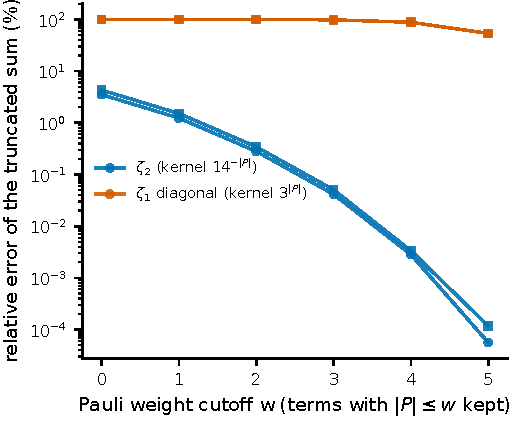
\includegraphics[width=0.62\linewidth]{fig10_weight_truncation}
\caption{The two projection variances read opposite ends of the Pauli spectrum. Relative error of each functional when its sum over Pauli strings is truncated to weight $|P| \leq w$, at $n = 6$ (circles noisy-pure, squares Haar-pure). $\zeta_2$ carries the kernel $14^{-|P|}$, which suppresses high weight, so a few percent of the strings determine it. The $\zeta_1$ diagonal carries $3^{|P|}$, which amplifies high weight, so most of the spectrum is needed. The cutoff $w = n$ is exact by construction and is not plotted.}
\label{fig:weights}
\end{figure}
\hypertarget{the-alpha-transition}{%
\subsection{\texorpdfstring{The \(\alpha\)
transition}{The \textbackslash alpha transition}}\label{the-alpha-transition}}

Fitting the sampled projection variances over this range gives clean
exponential scalings, retained here for the contrast with the closed forms
of Section~\ref{sec:zeta-closed-form} (which returns \(5.18\) for the
\(M^*\) base over this window against the regression's \(5.14\)).
Over \(n = 2\) to \(7\),

\[\zeta_1 \approx 0.63 \cdot (1.35)^n, \qquad \zeta_2 \approx 1.10 \cdot (6.93)^n, \qquad M^* \approx 0.87 \cdot (5.15)^n,\]

and over \(n = 2\) to \(9\), \(M^* \approx 0.76 \cdot (5.345)^n\); the
\(\zeta_1\) base is mildly curved, about \(1.35\) at small \(n\) and
\(1.30\) over the full range, which accounts for the difference. The
kernel variance grows roughly five times faster per qubit than the linear
variance, so their ratio \(M^*\) grows approximately exponentially over
the range we fit. The consequence is direct: at fixed budget, increasing
\(n\) pushes \(M\) below \(M^*\), the higher-order term takes over, and the
effective exponent \(\alpha\), the negative slope of
\(\log \mathrm{RMSE}\) against \(\log M\), fitted over the budget range
used (Appendix C), so window-averaged and shifting with \(n\), migrates
from \(1/2\) toward \(1\), and past it for higher \(k\):

\begin{table}[htbp]
\centering
\setlength{\tabcolsep}{10pt}
\begin{tabular}{@{}llll@{}}
\toprule
\(n\) & \(M^*(n)\) & predicted \(\alpha\) & measured \(\alpha\) \\
\midrule
2 & \(\approx 25.6\) & 0.501 & \(0.495 \pm 0.013\) \\
4 & \(\approx 549\) & 0.528 & \(0.528 \pm 0.012\) \\
9 & \(\approx 3.0 \times 10^{6}\) & 0.998 & \(1.006 \pm 0.023\) \\
\bottomrule
\end{tabular}
\end{table}

The \(M^*(n)\) column is the exact threshold evaluated from the
closed-form projection variances, not the fitted law evaluated at \(n\).
The predictions are computed from the projection variances (closed-form
at second order, estimated from shadow snapshots at higher) fed into
the exact variance formula, with nothing fitted to the \(\alpha\) data
(Fig.~\ref{fig:alpha}): the derived law matches 8 of 8 within two standard
errors at \(k = 2\), 6 of 7 at \(k = 3\) with the single miss on the
two-sigma boundary and seed-sensitive, and 5 of 5 at \(k = 4\).

The exact combinatorial structure is necessary, though \(k = 2\) is the
wrong place to see it. There the large-\(M\) truncation of Section 3.2,
\(\mathrm{Var} \approx 4\zeta_1/M + 2\zeta_2/M^2\), tracks the exact
variance to within 0.05\% across the budgets used and reproduces the
measured \(\alpha\) at 8 of 8, because at \(k = 2\) the second projection
and the full kernel variance coincide and the truncation discards nothing.
They separate at higher orders: keeping the same two terms with their
correct coefficients,
\(k^2\zeta_1/M + \tfrac{1}{2}k^2(k-1)^2\zeta_2/M^2\), gives 15 of 20
across \(k = 2, 3, 4\) against the exact law's 19 of 20, and misses
\(k = 3\), \(n = 8\) by twenty-six standard errors: by then
\(\zeta_3/\zeta_2\) exceeds \(10^4\) and the discarded terms carry the
variance.

A log-linear regression of \(M^*(n)\) over \(n = 2\) to \(9\) returns base
\(5.34\), 95\% CI \([5.14,\, 5.54]\), prefactor \(0.75 \pm 0.09\), and
\(\zeta_1, \zeta_2\) fit to bases \(1.30\ [1.26, 1.34]\) and
\(6.94\ [6.90, 6.98]\); the \(\zeta_2\) base sits just below the exact
per-qubit \(7\) at the maximally mixed state (Section 3.3) and barely
moves across windows, the drift carried by
\(\zeta_1\), in the manner Section~\ref{sec:zeta-closed-form} anticipates.
Appendix C gives the residual and leave-one-out detail.

\begin{figure}[tb]
\centering
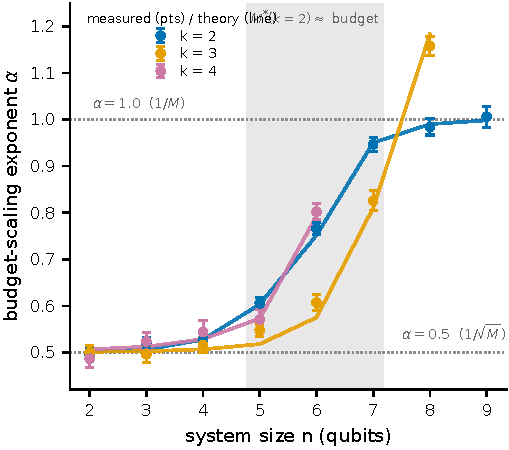
\includegraphics[width=0.74\linewidth]{fig3_alpha_transition}
\caption{The effective budget-scaling exponent transition, the paper's central phenomenon. Measured budget-scaling exponent $\alpha$ (RMSE $\propto M^{-\alpha}$, fitted over budgets $2000$--$128000$; markers with bootstrap standard errors) versus system size $n$ for moment orders $k=2,3,4$, with the derived-law prediction (lines). \emph{The prediction curves have no parameters fitted to the plotted points, computed from projection variances fed into the exact variance formula of Sec.~3.1, and are not fits to the plotted points.} As $n$ grows at fixed budget and $M$ falls below the threshold $M^*$, $\alpha$ migrates continuously from $1/2$ toward $1$, and past it for the higher moment orders.}
\label{fig:alpha}
\end{figure}

A fixed-exponent bound \(\mathrm{RMSE} \leq C_n/\sqrt{M}\) is not wrong; it
holds, and the tighter two-term treatments do not assume a fixed exponent
either \cite{elben2020mixed}. What it describes is the wrong regime for the
systems being run. At nine qubits and accessible budgets the estimator
sits near \(\alpha = 1\), where extra shots reduce error faster than
\(1/\sqrt{M}\) but from a variance already exponentially large, so any
extrapolation presuming \(\alpha = 1/2\) errs predictably. At fixed \(n\)
the linear term dominates once the budget grows without bound, so the
asymptotic scaling remains the square-root law: the migration reported
here is a finite-budget effect over the window hardware reaches, not a
change in asymptotic sample complexity.

Having characterized the single-copy cost exactly, we turn to the
collective route, where the error has a different character entirely.

\begin{center}\rule{0.5\linewidth}{0.5pt}\end{center}

\hypertarget{statewise-validation}{%
\section{Statewise validation}\label{sec:statewise}}

Section~3 makes a statewise claim: \(\zeta_1(\rho)\) and \(\zeta_2(\rho)\) are functionals of a
particular state, so they should predict what \emph{that} state does, not only what its family
does on average. Testing that is harder than it looks, and most of this section is about the
obstacle rather than the result.

\hypertarget{what-a-statewise-test-requires}{%
\subsection{What a statewise test requires}\label{what-a-statewise-test-requires}}

A cell of states can discriminate a statewise law from a family-average law only if the law's
predictions actually differ across the states in it, by more than the noise on the measurement
they are compared against. Write \(s\) for the relative spread of the predicted RMSE across a
cell and \(\eta\) for the relative noise on each measured RMSE; the cell is informative only when
\(s/\eta > 1\). On the four ensembles the crossover sweeps use, it is not:

\begin{center}
\begin{tabular}{lccccc}
\hline
state family & estimand & \(M^*\) max/min & \(s\) & \(\eta\) & \(s/\eta\) \\
\hline
Haar-pure          & fixed   & \(1.20\) & \(2.4\%\)  & \(5.9\%\)  & \(0.40\) \\
low-rank (rank 2)  & \(6.0\%\) & \(1.42\) & \(3.5\%\)  & \(5.9\%\)  & \(0.59\) \\
GHZ-noisy          & fixed   & \(1.00\) & \(0\)      & \(11.8\%\) & \(0\) \\
\hline
variable-\(q\)     & \(21.6\%\) & \(2.54\) & \(8.8\%\)  & \(5.9\%\)  & \(1.49\) \\
variable-rank      & \(73.8\%\) & \(9.74\) & \(27.0\%\) & \(5.9\%\)  & \(4.58\) \\
\hline
\end{tabular}
\end{center}

\noindent
at \(n = 4\), with \(s\) computed from the exact statewise variances and \(\eta\) from the trial
count of the sweep. The reason is structural, not a matter of effort. For the noisy-pure family
\(\mathrm{Tr}(\rho^k)\) is a function of \((n, q, k)\) alone and does not depend on
\(|\psi\rangle\), so the estimand is identical across the family and the projection variances
vary by a few percent; GHZ-noisy is a single state, so its spread is exactly zero. No affordable
trial count rescues them: at \(1.20\) between the extreme thresholds there is almost nothing to
order.

We therefore added two families whose parameters are drawn per state rather than fixed:
variable-\(q\), which is the noisy-pure construction with \(q \sim U[0.05, 0.45]\) drawn for each
state, and variable-rank, a Ginibre state of rank drawn uniformly from \(1\) to \(8\). Both cost
exactly what their fixed-parameter counterparts cost to sample. Variable-rank spans nearly a
factor of ten in statewise \(M^*\) and three quarters of its mean in the estimand itself, which
is what makes a statewise test possible at all.

\hypertarget{the-law-orders-individual-states}{%
\subsection{The law orders individual states}\label{the-law-orders-individual-states}}

On variable-rank at \(n = 3, 4, 5\), two budgets, \(14\) states per cell and \(300\)
forward-simulation trials per state --- so \(\eta \approx 4.1\%\) against a predicted spread of
\(21.9\%\) --- the exact statewise law reproduces each state's RMSE with a median relative
deviation of \(2.7\%\), and \(82\) of \(84\) state-budget pairs agree within two standard errors.
The ordering is recovered, not just the scale: the rank correlation between predicted and measured
RMSE within a cell averages \(\rho = +0.87\) with a minimum of \(+0.49\), and regressing measured
on predicted gives a slope of \(0.97\), a one-to-one relation across the decade the family spans
(Fig.~\ref{fig:statewise}, left).

The same run on noisy-pure is the control, and it behaves as the diagnostic says it must: the
median deviation is comparable at \(2.4\%\) and \(79\) of \(84\) pairs agree within two standard
errors, but \(\rho = +0.26\) and the slope is \(0.55\), because with \(s/\eta = 0.51\) there is no
ordering to recover (Fig.~\ref{fig:statewise}, right). A law that read only the family mean would
score the same there. Reporting the control alongside is the point: it is what distinguishes a
statewise result from an average one, and it is why the earlier sweeps, run entirely on
fixed-estimand families, could not have established this.

\begin{figure}[tb]
\centering
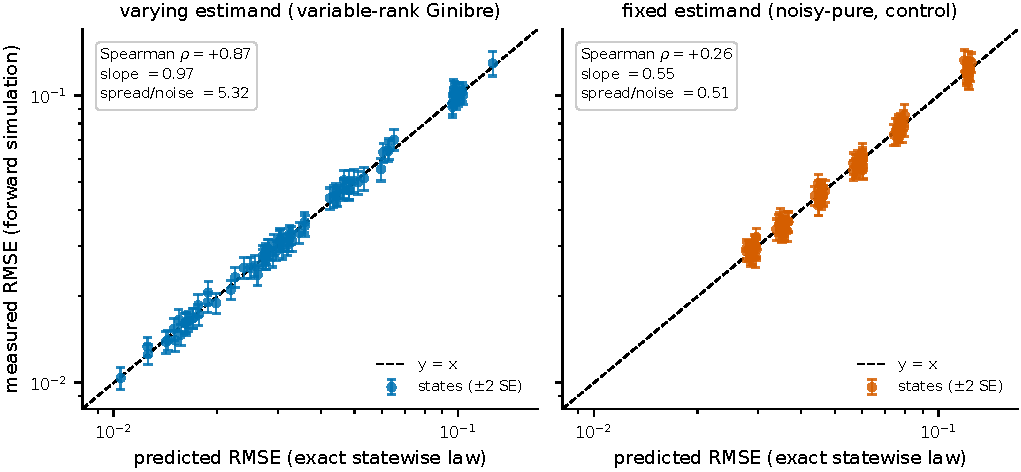
\includegraphics[width=\linewidth]{fig7_statewise_validation}
\caption{Statewise validation. Predicted versus measured single-copy RMSE for individual states at $k=2$, $n=3,4,5$ and two budgets, 14 states per cell, 300 trials each. \emph{Predictions come from each state's exact $\zeta_1,\zeta_2$, with nothing fitted to the plotted points.} Left: a varying-estimand family, where the statewise threshold spans an order of magnitude, so the law is tested state by state. Right: the fixed-estimand noisy-pure family as a negative control; its statewise spread is below the measurement noise, so no ordering can be resolved and a family-average law would score the same. Both panels share one scale.}
\label{fig:statewise}
\end{figure}

Two weaker statewise checks run over a wider grid, six families and \(n = 2\) to \(6\) at three
budgets with \(24\) trials each. There the exact law predicts per-state RMSE to a median
\(9.4\%\), consistent with the \(14\%\) trial noise of that run, with \(562\) of \(615\)
state-budget points inside two standard errors, and the per-state budget-scaling exponent within
two standard errors in \(194\) of \(205\) cases. Carrying one seed across sizes to form state
\emph{sequences}, since a single state lives at one size and cannot cross over by itself, the
criterion places the crossover exactly in \(82\) of \(123\) sequence-channel cells and within one
qubit in all \(123\). The exact rate is lower than the family-aggregate figures of
Section~\ref{validation-on-83-cells-and-four-ensembles}, which is the honest cost of asking a sharper question.

\hypertarget{the-crossover-sweep-on-the-new-families}{%
\subsection{The crossover sweep on the new families}\label{the-crossover-sweep-on-the-new-families}}

Adding the two families to the held-out crossover sweep extends it from three ensembles to five,
\(45\) swept cells at \(k = 2\) over three channels and three rates. Three checks fix the
comparison to what was already committed: the measured crossover on the original three ensembles
reproduces the earlier sweep in all \(27\) cells for the unbiased estimator and all \(27\) for
the range-projected one, and substituting the exact statewise projection variances for the
sampled ones on the prediction side moves the predicted crossover in none of the \(27\). The
exact evaluator is therefore free to adopt: it changes no number the earlier sweeps reported.

Over all five families the criterion resolves \(27\) crossovers and places \(26\) exactly and all
\(27\) within one qubit for the unbiased estimator, and \(26\) resolving with \(21\) exact and all
\(26\) within one for the range-projected estimator; scoring the non-crossing cells as
predictions as well gives \(42\) of \(45\) under either estimator. On the two new families alone
the unbiased figures are \(12\) resolving, all \(12\) exact, and \(18\) of \(18\) once
non-crossing cells are counted.

\begin{center}\rule{0.5\linewidth}{0.5pt}\end{center}

\hypertarget{estimating-the-threshold-from-a-pilot-budget}{%
\section{Estimating the threshold from a pilot budget}\label{sec:pilot}}

The threshold is exact but its inputs are the state, and an experimenter has snapshots. This
section closes that gap: \(M^*\) can be estimated from the snapshots themselves, without ever
forming the Pauli spectrum whose high-weight part Section~\ref{sec:evaluation-cost} shows is both
necessary to \(\zeta_1\) and badly estimated by shadows. The route around that is to estimate the
two variances \emph{as variances} rather than through their spectral representations.

\hypertarget{four-blocks-and-two-unbiased-estimates}{%
\subsection{Four blocks and two unbiased estimates}\label{four-blocks-and-two-unbiased-estimates}}

Split a pilot of \(M\) snapshots into four disjoint blocks \(A, B, C, D\) and write
\(K_{ij} = \mathrm{Tr}(G_i G_j) = \prod_q \mathrm{Tr}(G_i^q G_j^q)\). Then

\begin{itemize}
\tightlist
\item \(\zeta_2 = \mathrm{Var}[K_{ij}]\) is estimated by the sample variance of \(K\) over the
disjoint pairs \((A_i, B_i)\). Each pair is independent, so this is unbiased directly.
\item \(\mathbb{E}[\mathrm{Tr}(G\rho)^2]\) is estimated by
\(\mathrm{mean}_{i \in A}\, \bar K_{iB}\,\bar K_{iC}\) with
\(\bar K_{iB} = \mathrm{mean}_{j\in B} K_{ij}\). Because \(B\) and \(C\) are disjoint from each
other and from \(A\), the two inner means are independent unbiased estimates of
\(\mathrm{Tr}(G_i\rho)\), so their product is unbiased for \(\mathrm{Tr}(G_i\rho)^2\).
\item \(\mathrm{Tr}(\rho^2)^2\) is estimated by \(\bar K_{AB}\,\bar K_{CD}\) over the four
disjoint blocks, unbiased because the factors are independent and each is unbiased for
\(\mathrm{Tr}(\rho^2)\).
\item \(\zeta_1\) is the difference of the previous two.
\end{itemize}

Nothing here is a plug-in approximation; each piece is exactly unbiased, which is what lets a
small pilot be believed. Every block mean the construction needs is a mean of the
\(4^n\)-dimensional vector \(x_i = \bigotimes_q a_i^q\) of per-qubit Pauli coefficients, since
\(\mathrm{Tr}(G_iG_j) = 2^n \langle x_i, x_j\rangle\) for Hermitian factors, so the whole
computation is \(O(M 4^n)\) with no pairwise matrix ever formed.

The structure also says which factor will be hard. \(\zeta_1\) is a difference of two estimates
sharing the scale \(\mathrm{Tr}(\rho^2)^2\), each carrying noise of order \(\zeta_2/M\); since
\(\zeta_2\) grows as \(7^n\) while \(\zeta_1\) grows as \(\beta^n\) with \(\beta = 5/4\), the
difference is taken between quantities whose common part dominates. That is what the measurements
show: at \(n = 8\) and a pilot of \(32{,}000\) the relative error of \(\hat\zeta_2\) is
\(12.7\%\) while that of \(\hat\zeta_1\) is \(205\%\), and \(\hat\zeta_1\) comes out non-positive
in \(17\) of \(48\) draws, in which case the ratio is undefined rather than large and we report it
as such.

\hypertarget{how-much-pilot-it-takes}{%
\subsection{How much pilot it takes}\label{how-much-pilot-it-takes}}

Table~\ref{tab:pilot} gives the median relative error of \(\widehat{M^*}\) against the exact
statewise \(M^*\) for the same state, on the noisy-pure family. The error falls close to
\(M^{-1/2}\), as an unbiased variance estimate should, and the budget needed for a given accuracy
grows with \(n\) --- but much more slowly than the threshold it is locating.

\begin{table}[htbp]
\centering
\setlength{\tabcolsep}{9pt}
\begin{tabular}{@{}rrrrr@{}}
\toprule
\(n\) & \(M^*\) & \(10\%\) budget & ratio & error at that budget \\
\midrule
\(2\) & \(26\)        & \(8{,}000\)   & \(307\)   & \(5.5\%\) \\
\(3\) & \(110\)       & \(8{,}000\)   & \(72.6\)  & \(6.5\%\) \\
\(4\) & \(541\)       & \(8{,}000\)   & \(14.8\)  & \(8.8\%\) \\
\(5\) & \(2{,}884\)   & \(32{,}000\)  & \(11.1\)  & \(5.8\%\) \\
\(6\) & \(16{,}519\)  & \(32{,}000\)  & \(1.94\)  & \(9.0\%\) \\
\(7\) & \(91{,}741\)  & \(128{,}000\) & \(1.40\)  & \(8.4\%\) \\
\(8\) & \(520{,}955\) & \(512{,}000\) & \(0.98\)  & \(5.7\%\) \\
\bottomrule
\end{tabular}
\caption{Pilot cost against the threshold it locates, noisy-pure ensemble. The \(10\%\) budget is the smallest \emph{swept} budget whose median relative error on \(\widehat{M^*}\) fell below \(10\%\), so it is an upper bound set by the granularity of the grid and not an interpolation; the last column gives the error actually achieved there. Full error-versus-budget curves are in Fig.~\ref{fig:pilotratio}. The ratio crosses unity between \(n = 7\) and \(n = 8\).}
\label{tab:pilot}
\end{table}

The comparison that matters is against \(M^*\) itself, since a pilot larger than the threshold it
locates would be self-defeating. Measured, the ratio of the \(10\%\) budget to \(M^*\) falls from
\(\approx\!300\) at \(n = 2\) through \(1.94\) at \(n = 6\) and \(1.40\) at \(n = 7\) to
\(0.98\) at \(n = 8\): the pilot budget grows about twofold per qubit against the threshold's
roughly fivefold, so the overhead becomes relatively cheaper as \(n\) grows, and it crosses unity
between \(n = 7\) and \(n = 8\). Interpolating log-linearly between those two bracketing measured
points puts the crossing at \(n \approx 7.9\) (Fig.~\ref{fig:pilotratio}). We state this as
measured rather than extrapolated because an earlier fit over \(n \le 6\) alone put it near
\(n = 7\) while understating the required budget by a factor of \(1.85\) at \(n = 7\) and
\(3.8\) at \(n = 8\); the crossing survives that correction only because \(M^*\) grows
faster than the pilot does.

The tail of that convergence was worth a second look, because it is where an unbiased estimator
can still mislead. At sixteen repetitions the last octave at \(n = 8\) appeared to flatten,
falling only from \(8.4\%\) to \(7.3\%\), which is what an error floor would look like. It is not
one. Re-running the three largest budgets on independent states at forty repetitions --- \(120\)
pooled draws each --- gives \(27.7\%\), \(10.9\%\) and \(5.7\%\), a fitted exponent of \(-1.14\)
with a \(95\%\) confidence interval of \([-1.38, -0.88]\). That is at least as steep as the
\(M^{-1/2}\) an unbiased variance estimate should show, and it excludes the flattening: the
earlier appearance was an artifact of the repetition count. The median of \(\widehat{M^*}\)
relative to \(M^*\) over the same three budgets is \(1.059\), \(0.963\) and \(1.009\), scattering
about unity rather than settling at an offset, which is the other signature a floor would leave
and does not.

The higher-precision run does move one number, and we report the conservative reading. Its median
deviation at \(256{,}000\) is \(10.9\%\) rather than the \(8.4\%\) the sixteen-repetition run
gave, so that budget now sits just above the \(10\%\) line and the bracket at \(n = 8\) becomes
\(512{,}000\). Two independent determinations straddle the threshold there, which is precisely
the grid-granularity fragility Table~\ref{tab:pilot} is caveated for; taking the larger moves the
ratio at \(n = 8\) from \(0.49\) to \(0.98\) and the crossing from \(n \approx 7.3\) to
\(n \approx 7.9\). Table~\ref{tab:pilot} and Fig.~\ref{fig:pilotratio} use the larger value. The
qualitative claim is unchanged --- the pilot cost falls below the threshold it locates by eight
qubits --- and we prefer the version that claims less. A bracket read off a doubling grid is a
coarse instrument near the threshold, and should be read as one.

The varying-estimand family is harder in absolute terms, and we report it separately rather than
pooled, because pooling would hide the reason. On variable-rank the \(10\%\) budget is
\(8{,}000\) at \(n = 2\), \(32{,}000\) at \(n = 4\), \(128{,}000\) at \(n = 6\), and more than
\(256{,}000\) at \(n = 7\), where the error is still \(19.7\%\) at that budget. But its thresholds
are correspondingly larger --- \(M^* = 503{,}444\) at \(n = 7\) against \(91{,}741\) for
noisy-pure --- so the two move together: rank-deficient states have smaller \(\zeta_1\), which
raises \(M^*\) and makes \(\zeta_1\) harder to estimate at once. The ratio, not the budget, is the
quantity that transfers.

\begin{figure}[tb]
\centering
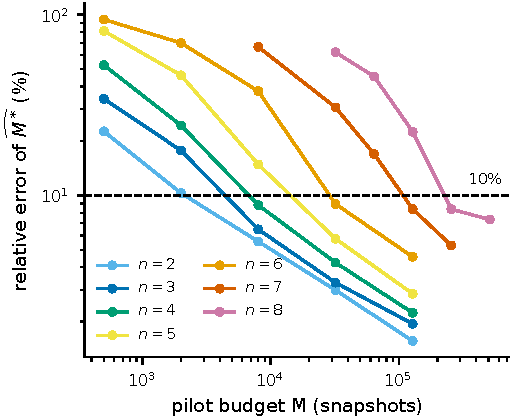
\includegraphics[width=0.9\linewidth]{fig8_pilot_convergence}\hfill
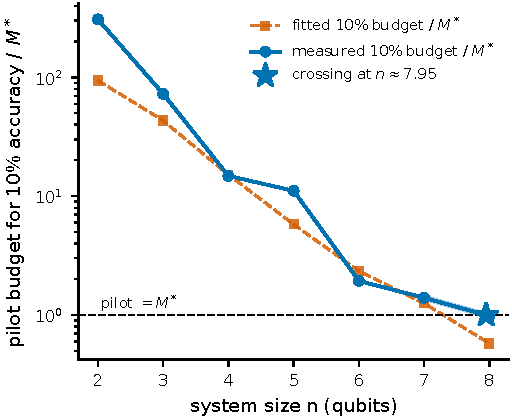
\includegraphics[width=0.9\linewidth]{fig9_pilot_over_mstar}
\caption{Estimating the threshold from data. \emph{Left:} median relative error of $\widehat{M^*}$ against the exact statewise $M^*$ versus pilot budget, noisy-pure, one curve per size; the dashed line marks $10\%$ accuracy. \emph{Right:} the $10\%$ budget relative to $M^*$ itself. Circles are the smallest swept budget that achieved $10\%$, so they are upper bounds set by the grid, which is why the first three coincide; squares are a log-log fit through the usable range. The star marks where the measured ratio crosses unity, interpolated between the two measured sizes that bracket it. Below the dashed line the pilot costs less than the threshold it locates.}
\label{fig:pilotratio}
\end{figure}

What this does not provide is a performance guarantee. The estimators are unbiased and their
convergence is measured, but bounding the probability that a pilot puts an experiment on the wrong
side of \(M^*\) needs a concentration bound for \(\hat\zeta_1\), which is a difference of degree-2
and degree-4 statistics in snapshots whose kernel variance grows as \(7^n\); the fourth moment
that a Bernstein-type argument would need is itself a higher-order projection variance we do not
have in closed form. We state the convergence we measured and leave the guarantee open.

\begin{center}\rule{0.5\linewidth}{0.5pt}\end{center}

\hypertarget{the-collective-route-two-exact-bias-laws}{%
\section{The collective route: two exact bias
laws}\label{the-collective-route-two-exact-bias-laws}}

At nonzero noise, once the shot budget is large enough that the
finite-shot term has decayed, the collective route's error is dominated
by a bias rather than a variance; at zero noise or small budgets the
finite-shot variance dominates instead. The bias is independent of the
shot budget, a prediction Section 7.4 tests directly and which holds.
Its functional form is fixed by the geometry of the noise channel, its
magnitude by geometry and rate together, and two channel classes give
two exact laws.

\hypertarget{global-depolarizing-noise-linear-in-g-with-no-compounding}{%
\subsection{\texorpdfstring{Global depolarizing noise: linear in
\(g\), with no
compounding}{Global depolarizing noise: linear in g, with no compounding}}\label{global-depolarizing-noise-linear-in-g-with-no-compounding}}

Let the \(kn\)-qubit collective register be subject to global
depolarizing noise at rate \(g\), so that
\(\rho^{\otimes k} \mapsto (1-g)\rho^{\otimes k} + g\,\mathbb{I}/d^k\)
with \(d = 2^n\). Then

\[\mathrm{Tr}\!\left( C_k \left[ (1-g)\rho^{\otimes k} + g\,\tfrac{\mathbb{I}}{d^k} \right] \right) = (1-g)\,\mathrm{Tr}(\rho^k) + g\,\frac{\mathrm{Tr}(C_k)}{d^k} = (1-g)\,\mathrm{Tr}(\rho^k) + g\, 2^{\,n(1-k)},\]

using \(\mathrm{Tr}(C_k) = d\) from Section 2.3. Hence

\[\boxed{\;\text{bias} = g \left| \mathrm{Tr}(\rho^k) - 2^{\,n(1-k)} \right| \;}\]

At a fixed \(g\) the bias is linear in \(g\) and does not compound
across qubits: the single-cycle property of \(C_k\) collapses the
compounding that a per-qubit form \(1 - (1-g)^{kn}\) would predict, and
which overestimates the bias by a factor of five to fourteen over the
range swept here. The two forms are parametrically different in \(n\),
the compounding form saturating toward unity while the true bias stays
linear. This holds at fixed \(g\); on hardware the effective global rate
may itself grow with register size, depth, or gate count.

\hypertarget{per-qubit-channels-the-noise-relabels-the-state}{%
\subsection{Per-qubit channels: the noise relabels the
state}\label{per-qubit-channels-the-noise-relabels-the-state}}

Let \(\mathcal{E}\) be any single-qubit channel borne by the collective
route and not by the single-copy route, applied to every qubit of every
copy held for the test, with \(\rho\) the reference state and
\(\mathrm{Tr}(\rho^k)\) the estimand. That \(\mathcal{E}\) is specific
to this route is a modeling choice rather than a derivation, and it is
what makes the quantity below a bias.

The identity needs one further precondition, and it is narrow: the
\(k\) copies must be independent and must undergo
\(\mathcal{E}^{\otimes n}\) \emph{before} an otherwise ideal
cyclic-permutation measurement. It does not cover noise inside the
cyclic test (imperfect controlled-permutation gates, ancilla
decoherence, readout error), nor correlated noise acting across
copies, nor any channel acting during or after the circuit. Those
perturb the measured observable or the instrument rather than the state
being measured, and the relabeling does not apply to them. Within that
precondition,

\[\mathcal{E}^{\otimes nk}\!\left( \rho^{\otimes k} \right) = \left( \mathcal{E}^{\otimes n}(\rho) \right)^{\otimes k} = \sigma^{\otimes k}, \qquad \sigma \equiv \mathcal{E}^{\otimes n}(\rho),\]

and the cyclic test of a product of identical states returns the
\(k\)-th moment of that state:

\[\boxed{\;\text{measured} = \mathrm{Tr}(\sigma^k), \qquad \sigma = \mathcal{E}^{\otimes n}(\rho) \;}\]

so the bias is
\(\left| \mathrm{Tr}(\sigma^k) - \mathrm{Tr}(\rho^k) \right|\). The
noise does not corrupt the measurement in the usual sense; it relabels
which state is measured, and that substitution is the entire bias. A
channel common to both routes would bias the single-copy route by the
same substitution and cancel from the comparison, carrying no
information about which route has the lower RMSE at equal state-copy
budget; the law requires that \(\mathcal{E}\) be borne by the collective
route alone. Preparation noise is not excluded but already absorbed into
\(\rho\) by the ensemble of Section 2.5, which both routes see and which
contributes no bias.

\hypertarget{verification}{%
\subsection{Verification}\label{verification}}

Both laws are exact identities rather than approximations, and we
verified them accordingly: against explicit construction of \(C_k\) and
the noise-damaged \(k\)-copy state, at \(n = 2, 3\) and \(k = 2, 3, 4\),
for global depolarizing, amplitude damping, and dephasing, agreeing to
approximately \(10^{-15}\). We take the single-qubit Kraus operators at
rate \(g\) in the standard form: amplitude damping as
\(K_0 = \mathrm{diag}(1, \sqrt{1-g})\) and
\(K_1 = \sqrt{g}\,\lvert 0 \rangle \langle 1 \rvert\); dephasing as
\(K_0 = \sqrt{1 - g/2}\,\mathbb{I}\) and \(K_1 = \sqrt{g/2}\,Z\); and
global depolarizing in the closed form of Section 6.1. Each is applied to
every qubit of every copy. They continue to hold at three times the
noise rates in which they were derived, and on state ensembles they had
never been tested against: Haar-pure (\(q = 0\)); low-rank,
\(\rho = GG^\dagger\) with \(G\) a \(2^n \times 2\) complex Ginibre
matrix normalized to unit trace, whose spectrum is not the
rank-one-plus-identity form the noisy-pure closed forms assume; and
GHZ-noisy,
\((1-q)\lvert \mathrm{GHZ} \rangle \langle \mathrm{GHZ} \rvert + q\,\mathbb{I}/2^n\)
at \(q = 0.15\) with
\(\lvert \mathrm{GHZ} \rangle = (\lvert 0 \cdots 0 \rangle + \lvert 1 \cdots 1 \rangle)/\sqrt{2}\).
An exact identity is not expected to degrade under extrapolation, and it
does not.

With the single-copy variance in closed form at \(k=2\) and the
collective bias an exact identity, the crossover follows by setting one
against the other.

\begin{center}\rule{0.5\linewidth}{0.5pt}\end{center}

\hypertarget{the-crossover}{%
\section{The crossover}\label{the-crossover}}

\hypertarget{the-law}{%
\subsection{The law}\label{the-law}}

The single-copy error of the unbiased estimator grows exponentially in
\(n\) and falls with the budget;
Section~\ref{physical-constraints-and-the-choice-of-estimator} takes up the
range-projected alternative, for which it instead saturates. The collective
error is a bias floor plus a finite-shot variance:
the floor is bounded above by \(1 - d^{1-k}\) with \(d = 2^n\), hence by
unity, and is independent of the budget, while the shot term vanishes as
the budget grows. The crossover size \(n^*\) is where the single-copy
error rises above the collective error,

\[\underbrace{\sqrt{\mathrm{Var}(U_M)}}_{\text{exponential in } n,\ \text{falls with } M} \;=\; \underbrace{\sqrt{\text{bias}(g, k, n)^2 + \frac{1 - \mu^2}{N}}}_{\text{bounded floor}\;+\;\text{shot noise}}\]

Here \(\mu\) is the noisy collective signal the cyclic test returns and
\(N = \lfloor M/k \rfloor\) is the number of \(k\)-copy measurements a
copy budget of \(M\) allows. The shot term is the variance of the bounded
cyclic-test outcome and falls away as the budget grows, leaving the bias
floor as the large-budget limit. Every quantity on both sides comes from
Sections 3 and 6; nothing is fitted to the data being predicted, and the
laws take the state's projection variances and the noise channel as
inputs.

The bounded-floor claim is a statement about bias in \emph{estimation} at
fixed additive precision \(\varepsilon\): the collective-test outcome is a
bounded random variable, so estimating \(\mathrm{Tr}(\rho^k)\) to fixed
\(\varepsilon\) costs \(O(1/\varepsilon^2)\) shots at every \(n\), and the
collective error saturates at the floor rather than growing. It is not a
claim that collective measurement is cheap for all tasks: for a task whose
target precision must itself shrink exponentially in \(n\),
\cite{noisylearning2026} proves that exponentially many samples are
required even with two copies. Section~8 gives the quantitative
reconciliation.

\hypertarget{validation-on-83-cells-and-four-ensembles}{%
\subsection{Validation on 83 cells and four
ensembles}\label{validation-on-83-cells-and-four-ensembles}}

Across 83 cells spanning moment order \(k \in \{2,3,4\}\), three noise
models (depolarizing, amplitude damping, dephasing), noise rates from 0 to
0.3, sizes \(n = 2\) to \(9\), four budget multipliers, and four state
ensembles, the criterion predicts 82 of the 83 simulated crossovers within
one qubit and 73 of 83 exactly (Figs.~\ref{fig:crossmap}
and~\ref{fig:boundary}). Those figures are for the unbiased U-statistic of
Section 3, the estimator the variance law describes. For the range-projected
estimator of Section~\ref{physical-constraints-and-the-choice-of-estimator},
11 cells stop resolving a crossover and the criterion places all 72 that
remain within one qubit, 63 of them exactly. Both are reported throughout:
they describe two different estimators, and neither supersedes the other.

Neither aggregate is homogeneous, and the split matters for reading it. The
83 are 68 noisy-pure cells whose measured \(n^*\) comes from the paired
state-level \(z\)-test against measured collective data, plus 15 held-out
cells whose measured \(n^*\) comes from the measured single-copy RMSE
against the theory collective floor; for the range-projected estimator the
72 are 58 and 14 of the same two kinds. Appendix~C states the three rules
and which produced which figures. The two subsets are therefore scored by
different rules, and the aggregate should be read as their union rather
than as one homogeneous sample.

The comparison is asymmetric between the routes in two respects, both
deliberate. The first is evidential: the single-copy side of each cell is
a forward simulation of the estimator, fresh snapshots reduced by the
U-statistic, so the variance law is tested against data it did not
generate, while the collective side is the exact bias law evaluated
analytically plus its shot noise.

The second is the noise model, and it is the stronger assumption. The
channel of Section 6 degrades the collective route only; the single-copy
route is the ideal, noiseless statistical baseline, on the reading that a
joint \(k\)-copy measurement is the harder thing to implement cleanly.
Real shadow readout is not noiseless, so this understates the single-copy
cost, in the direction that costs us. Simulating readout on both routes,
and correcting the collective parity for readout exactly through its
outcome-dependent per-pair contraction rather than a blanket factor, moves
the crossover to smaller \(n\) in every resolved cell. The magnitude of
that shift depends on device-specific per-qubit rates and is quantified in a
companion study of the hardware case; the direction is what matters here,
and the sizes reported below are therefore a conservative upper bound under
this noise model. Under
uncorrected readout the single-copy U-statistic acquires a bias that does
not shrink with the copy budget, unlike its noiseless variance, so both
routes then carry error floors and the comparison changes character. What
the asymmetry does shape is the dependence of \(n^*\) on the noise rate,
which is a property of the collective side by construction.

These cells demonstrate consistency with the derived identities; the
additional ensembles test whether the plug-in variance architecture stays
accurate when its projection-variance inputs are re-estimated outside the
derivation ensemble. What transfers is the structure of the formula, not
the noisy-pure coefficients, which are re-estimated for each ensemble, so
this is not zero-shot prediction from universal constants. Three of the four ensembles (Haar-pure,
low-rank, and GHZ-noisy) were never used in deriving the law. GHZ
states are maximally non-Haar-typical, and we included them because an
ensemble-tuned theory ought to fail on them; the theory's accuracy there
is within a factor of about 1.7 of its accuracy elsewhere, the same order
of magnitude rather than a breakdown. All four have a fixed estimand, which
is what makes them unsuitable for the statewise test of
Section~\ref{sec:statewise}; the extension of this sweep to two
varying-estimand families, and the checks tying it back to the counts
reported here, are in Section~\ref{the-crossover-sweep-on-the-new-families}.

\begin{figure}[tb]
\centering
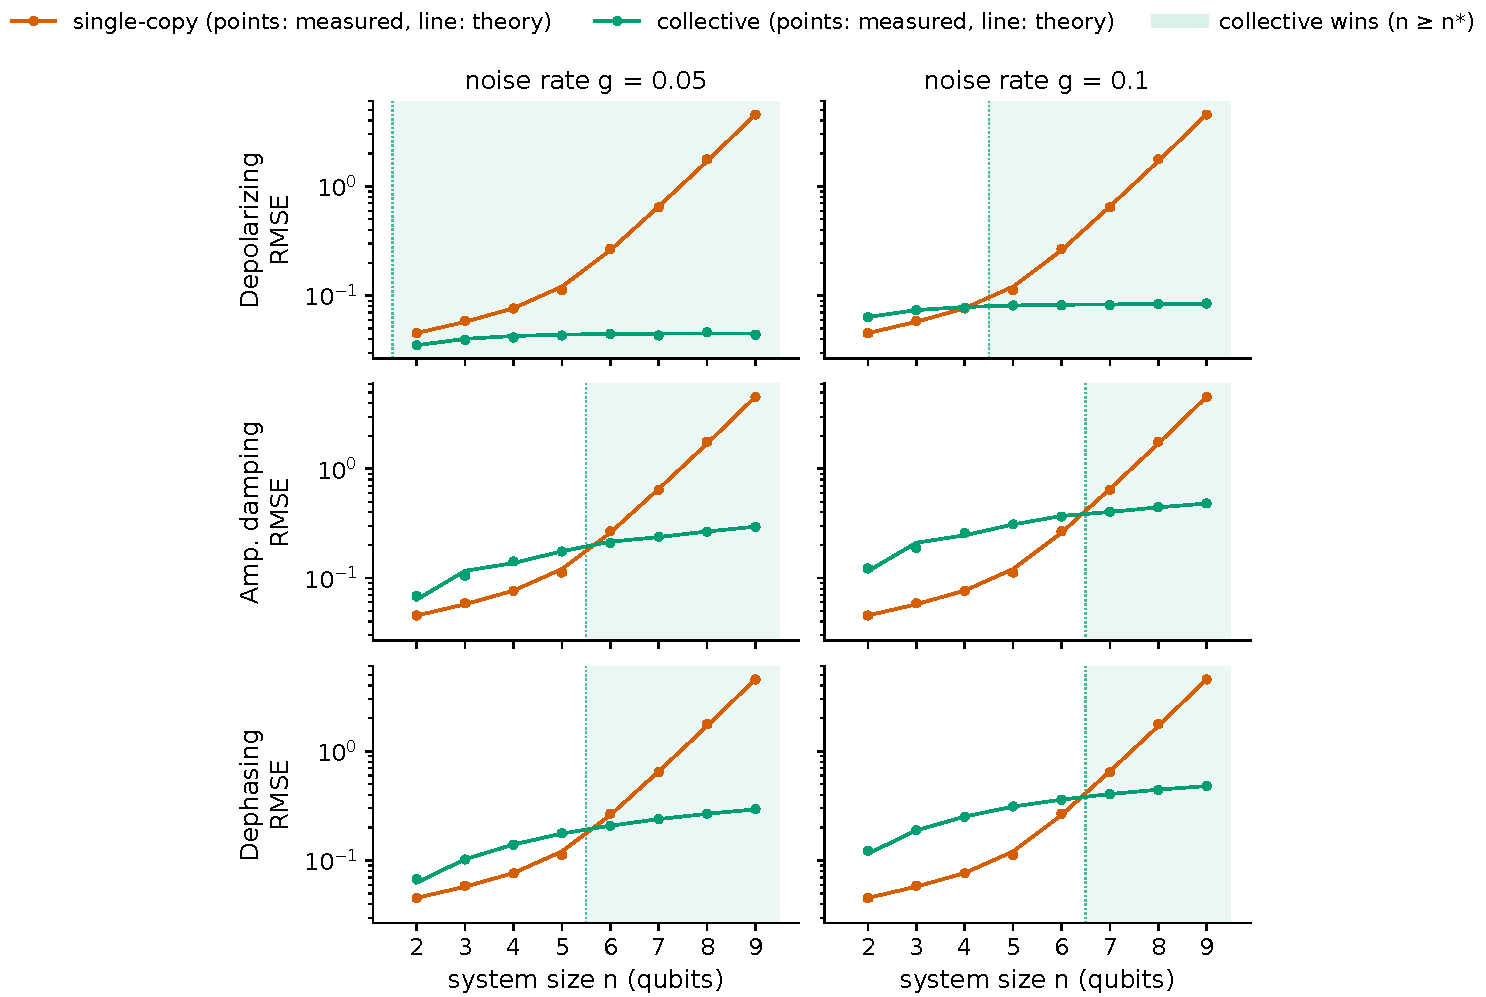
\includegraphics[width=0.74\linewidth]{fig1_crossover_map}
\caption{The crossover for purity ($k=2$). Single-copy classical-shadow RMSE (vermillion) and collective two-copy RMSE (green) versus system size $n$ at a fixed copy budget, for three noise channels. \emph{The theory curves are predictions with no parameters fitted to these points, from the exact variance and bias laws (Secs.~3 and~6), not fits to these points.} The crossover $n^*$ is where the exponentially growing single-copy error overtakes the collective error, a bounded bias floor plus a finite-shot variance that vanishes as the budget grows.}
\label{fig:crossmap}
\end{figure}

\begin{figure}[tb]
\centering
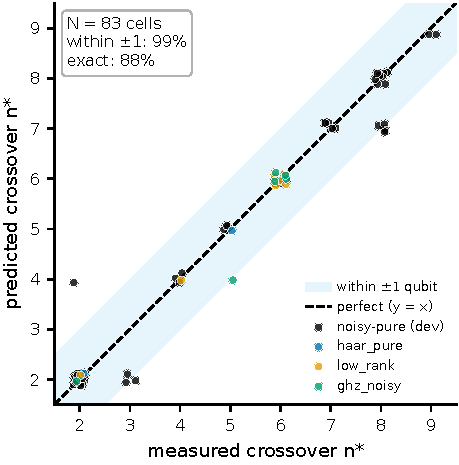
\includegraphics[width=0.74\linewidth]{fig2_crossover_boundary}
\caption{Crossover validation across 83 cells. Predicted versus Monte-Carlo-observed crossover size $n^*$ over moment orders $k\in\{2,3,4\}$, three noise models, and four state ensembles (three unseen by the theory). Accuracy for the unbiased estimator (83 resolving cells, as 68 noisy-pure plus 15 held-out) and for the range-projected estimator (72, as 58 plus 14) is reported in Secs.~7.2 and~7.3; the two subsets are scored by different rules (Appendix~C). The cells are simulation, not hardware; for the higher moment orders the collective side is an idealized bounded-outcome primitive carrying no gate, depth, or routing cost.}
\label{fig:boundary}
\end{figure}

\begin{figure}[tb]
\centering
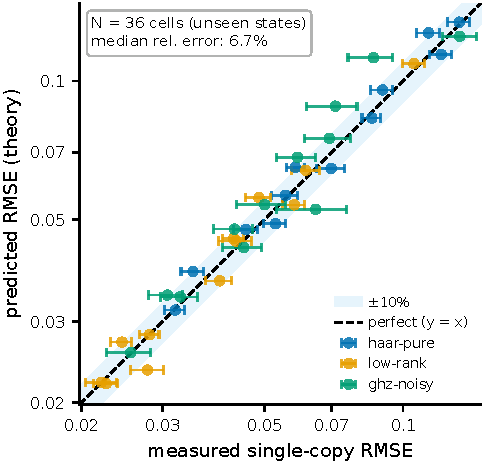
\includegraphics[width=0.74\linewidth]{fig4_out_of_ensemble}
\caption{Out-of-ensemble validation of the variance law. Predicted versus measured single-copy RMSE on three ensembles the theory never saw (Haar-pure, low-rank, GHZ-noisy). The scatter about the diagonal is finite-trial estimation noise (median relative deviation 6.7\%; Sec.~9), not a systematic error.}
\label{fig:ooe}
\end{figure}

\hypertarget{physical-constraints-and-the-choice-of-estimator}{%
\subsection{Physical constraints and the choice of
estimator}\label{physical-constraints-and-the-choice-of-estimator}}

Every moment obeys \(\mathrm{Tr}(\rho^k) \in [d^{1-k}, 1]\) with
\(d = 2^n\), a range fixed before any data is taken. An estimate falling
outside it can therefore be replaced by its Euclidean projection onto that
interval,

\[\widehat{U}^{\mathrm{c}}_M = \min\bigl\{\max\{\widehat{U}_M,\, d^{1-k}\},\, 1\bigr\},\]

a contraction onto a convex set containing the truth, which cannot increase
the squared error of any individual estimate, pointwise, with no
distributional assumption. Over 4320 samples spanning \(n = 2\) to \(10\) it
increased it zero times.

The effect is not marginal. On the headline configuration at \(n = 10\),
97.9\% of raw estimates fall outside the physical range, and projection cuts
the RMSE from 11.98 to 0.58, a factor of 20.6.

Section 3 is untouched by this. It gives the variance of the unbiased
U-statistic, and that remains accurate: the closed-form Hoeffding prediction
is 11.92 at \(n = 10\) against 11.976 measured. What changes is which
estimator an experimenter would actually use, and the criterion has to be
re-derived for that one.

Doing so and re-running the full sweep, the criterion predicts the crossover
size within one qubit in all 72 cells that resolve a crossover (100.0\%),
exactly in 63 of those 72 (87.5\%), and correctly on 119 of the 123 swept
cells (96.7\%) once non-crossing cells are scored as predictions, against
82 of 83, 73 of 83, and 118 of 123 for the unbiased estimator. The criterion
is more accurate under projection, not less. Bounding both errors compresses
the predicted and measured curves onto the same scale, so cells that
straddled the boundary in the unbounded comparison stop straddling it.

The cost is a smaller denominator, and it falls in one place. Projection
removes the crossover entirely from 11 cells, so 72 rather than 83 resolve;
the loss is all on noisy-pure (68 cells to 58) and GHZ-noisy (7 to 5). Where
a crossover survives it never moves earlier: 60 of the 72 are unchanged, 10
move one qubit later, and 2 move four. Haar-pure keeps both its cells, each
one qubit later; low-rank keeps all seven, unmoved.

Projection makes the single-copy estimator biased, so the comparison in
Section~\ref{the-law} is no longer an unbiased variance against a bias floor
but a comparison of two error floors. That is the same change of character
the readout simulation in
Section~\ref{validation-on-83-cells-and-four-ensembles} already imposes on
both routes, and as there it does not reverse the ordering the criterion
predicts.

\hypertarget{three-qualitative-predictions-and-the-one-we-got-wrong}{%
\subsection{Three qualitative predictions, and the one we got
wrong}\label{three-qualitative-predictions-and-the-one-we-got-wrong}}

Two of the three we predicted correctly in advance; the third we got
backwards, and the law corrected us.

Higher noise moves the crossover later on the channels and rates we swept:
a larger bias floor takes longer for the exponentially growing single-copy
error to climb over. A larger budget moves it later too, because the
single-copy error falls with budget while the bias floor does not; the
collective RMSE plateaus exactly at the predicted floor as the budget
grows while the single-copy RMSE keeps falling, a direct test of the
bias-versus-variance distinction on which the whole crossover rests.

Higher \(k\) also moves the crossover later on the families we tested, and
this is counterintuitive: a naive variance argument says higher moments
compound the single-copy variance faster and should cross earlier. The law
explains the reversal. \(\mathrm{Tr}(\rho^k)\) shrinks with \(k\), so the
absolute bias floor the single-copy error must climb over is lower, and
single-copy holds out to larger \(n\). We report this as an observation
about the ensembles and channels swept here rather than a general rule:
\(\lvert \mathrm{Tr}(\sigma^k) - \mathrm{Tr}(\rho^k) \rvert\) need not
fall monotonically with \(k\) for an arbitrary spectrum and channel. No
universal effective attenuation rate fits the measured biases either,
because the bias is not a rate: it is however much the channel deforms
that particular state's spectrum, and two states of identical purity can
be deformed by different amounts. Purity (\(k=2\)) crosses at
\(n \approx 6\) to \(7\) under realistic noise, while \(k = 3\) and
\(k = 4\) hold out to \(n \approx 8\), sizes for the idealized
bounded-outcome test of Section 2.3, whose realization costs about an
order of magnitude more two-qubit gates than the \(k = 2\) test, plus an
ancilla and routing. The signal-against-a-fixed-floor argument dominates
the variance-compounding argument.

\hypertarget{where-single-copy-estimation-stops-being-useful}{%
\subsection{Where single-copy estimation stops being
useful}\label{where-single-copy-estimation-stops-being-useful}}

The practical statement is a single sequence. Using the exact copy-fair
unbiased estimator on noisy-pure states at a fixed copy budget, the
single-copy purity RMSE runs

\[0.043 \;\to\; 0.072 \;\to\; 0.270 \;\to\; 1.62 \;\to\; 11.98\]

at \(n = 2, 4, 6, 8, 10\), growing by a factor of about two per qubit on
average and accelerating to roughly 2.7 per qubit over the last step,
against a true purity of approximately 0.81 (Fig.~\ref{fig:wall}).
Projected into the physical range as in
Section~\ref{physical-constraints-and-the-choice-of-estimator}, the same
estimates give 0.043, 0.071, 0.227, 0.500, 0.582: bounded, and saturating
rather than diverging.

The bounded sequence carries the sharper statement, because it no longer
rests on an unbounded scale. A constant fixed at the midpoint of
\([2^{-n}, 1]\), the interval the purity is known a priori to occupy,
and all that a guess which never looks at the data can use, has RMSE
0.308 at \(n = 7\) against the projected single-copy estimator's 0.400, and
0.310 at \(n = 10\) against its 0.582. From seven qubits on, the
single-copy route is worse than that constant. The collective route holds
out three qubits longer, beating the same constant through \(n = 9\) and
falling behind it only at \(n = 10\) (0.320 against 0.310). The collective
route stays
bounded over the same range, because its error is a bias floor and the
floor cannot exceed \(1 - d^{1-k} < 1\): both \(\mathrm{Tr}(\sigma^k)\)
and \(\mathrm{Tr}(\rho^k)\) lie in \([d^{1-k}, 1]\), so their difference
is bounded by the width of that interval. What is universal is the weaker
statement that the floor stays below unity, and that is what the crossover
argument uses.

This speaks to the resource-cost concern behind the choice in
\cite{qmladvantage2026} to keep its measure-first protocol single-copy.
The entangling overhead that motivates such caution is real, and it is not
the binding constraint. The binding constraint is that at the tested budgets
the local-randomized-measurement shadow U-statistic we study becomes
statistically unusable for moment estimation at comparable system sizes,
a statement about this protocol, not about every single-copy
strategy.

\begin{figure}[tb]
\centering
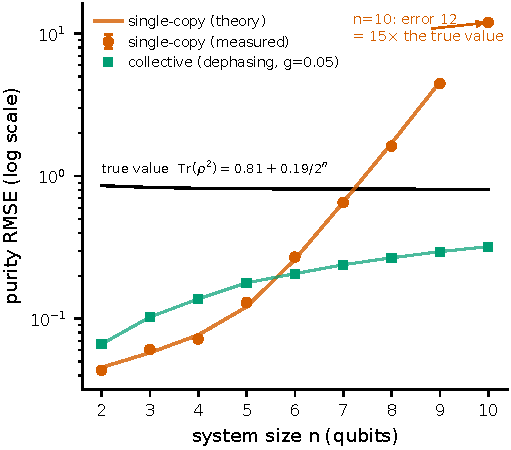
\includegraphics[width=0.72\linewidth]{fig5_exponential_wall}
\caption{Single-copy error growth against a bounded collective error. Single-copy purity RMSE for the unbiased U-statistic versus $n$ out to $n=10$ at a fixed copy budget of $M=2000$ (log scale; measured points with 68\% CIs, theory line with no parameters fitted to the crossover data; noisy-pure ensemble, collective route under dephasing at $g=0.05$), with the exact per-$n$ true purity $\mathrm{Tr}(\rho^2)=0.81+0.19/2^{n}$ marked ($0.858$ at $n=2$, approaching $0.81$). By $n=10$ the single-copy error reaches $\sim\!12$ while the collective error (green) stays bounded. Projecting the single-copy estimate into the physical range (Sec.~7.3) caps it at $0.582$, but does not restore its usefulness: from $n=7$ on it is beaten by a constant fixed at the midpoint of that range, which uses no data at all.}
\label{fig:wall}
\end{figure}

\begin{center}\rule{0.5\linewidth}{0.5pt}\end{center}

\hypertarget{related-work}{%
\section{Related work}\label{related-work}}

\textbf{Classical shadows and variance bounds.} The classical-shadow
framework \cite{huang2020shadows} gives sample-complexity bounds via the
shadow norm; for second-order nonlinear functionals the variance splits
into a kernel term bounded by \(4^{|AB|}\) and linear terms bounded by
\(2^{|AB|}\) \cite{shadownorm2021}, which states and applies the bound
citing its own references, so we attribute the statement rather than its
origin. These are worst-case, state-independent bounds. For local
randomized measurements, Huang, Wang and Xu \cite{huang2026worstcase} give
worst-case bounds whose exponential base depends on the measurement
ensemble, for the related task of distributed inner-product estimation;
these remain envelopes rather than evaluated coefficients or a threshold,
as do the companion bounds for structured circuits below a 4-design
\cite{zheng2026structured}.
The exact finite-\(M\) decomposition is the standard Hoeffding identity
\cite{hoeffding1948, serfling1980}, already stated as an equality for
shadows by \cite{huang2020shadows} and again by Elben et
al.~\cite{elben2020mixed}, who read the two-regime scaling off it.
Reference \cite{elben2020mixed} bounds \(\zeta_1\) and \(\zeta_2\) rather
than evaluating them; \cite{huang2020shadows} does supply the exact second
moment, in its Lemma 4, but applies it to worst-case sample complexity
rather than evaluating the coefficients for a state or an ensemble.
Neither gives a threshold in \(M\), and separate upper bounds constrain
the ratio not at all, which is why the threshold does not follow from
them. What this work adds is the evaluation of
Section~\ref{sec:zeta-closed-form}, the resulting threshold, the spectral
functionals fixing its growth base, and the comparison against the
collective route. Alternative shadow ensembles
\cite{hamiltonianshadow2021} target different observable classes.
Deliberately biased shadow estimators have been studied directly:
\cite{cai2025biased} rescales the estimator by a tuned factor, shrinking it
toward zero, and argues the trade is always worth making in the
finite-sample regime. The projection of
Section~\ref{physical-constraints-and-the-choice-of-estimator} accepts bias
for the same reason but by a different mechanism: it has no free parameter
and no shrinkage target, and moves an estimate only when that estimate is
infeasible. That an estimator reporting values on the boundary of the
feasible set can itself be improved by hedging inward is known from
tomography \cite{ferrie2018inadmissible}.

\textbf{U-statistics and the Hoeffding decomposition for quantum
moments.} Straeter, Tsesmelis and Kwek \cite{straeter2026} construct
unbiased U-statistic estimators for the partial-transpose moments \(p_2\)
and \(p_3\) from randomized homodyne data and derive their variance via a
Hoeffding decomposition, obtaining sample-complexity bounds for a
\(p_3\)-PPT entanglement criterion. This is the closest methodological
neighbor to Section 3; the differences are the platform, the target
(entanglement detection rather than moment estimation and the
collective-measurement trade-off), and the result, since their projection
variances are bounded rather than evaluated for a state and no change of
scaling regime is considered. Two further analyses treat the shadow
U-statistic itself. Jnane et al.~\cite{jnane2024mitigated} write the exact
Lee variance for U-statistics of shadow snapshots, then bound the
projection terms by a quasiprobability norm and keep only the leading
\(1/N\), the step that hides the second regime. Pelecanos et
al.~\cite{pelecanos2025spectrum} study the same estimator for
\(\mathrm{Tr}(\sigma^k)\) under the uniform POVM and prove an explicit
variance bound for it; that bound is an inequality in \(d\) for a
worst-case state rather than an evaluation for an ensemble, and locates no
threshold. We claim no novelty for the Hoeffding
technique itself.

\textbf{Crossovers, hybrids, and cheaper collective routes.} A crossover in
shot cost between Pauli and Clifford shadow ensembles has been reported for
multipartite entanglement witnesses \cite{paulicliffordxover2026}; that is a
crossover in the choice of measurement ensemble, not between single-copy and
collective measurement. Zhou and Liu \cite{zhou2024hybrid} interpolate
between the routes instead of choosing, applying randomized measurements to
a few coherently prepared copies; the measurement counts they report order
the protocols without locating a size at which the ordering changes. A
parallel line lowers the cost of the collective route itself
\cite{shin2025resource, shi2025moments, yao2026sample}, through
Newton--Girard recursions, qubit reuse, or coherent evaluation of the
functional; these improve the side our criterion compares against rather
than moving where it crosses.

\textbf{Sample-complexity lower bounds for purity.} Gong et
al.~\cite{gong2024purity} improve the lower bound for purity estimation to
\(\Omega(\max\{1/\varepsilon^2,\, 2^{n/2}/\varepsilon\})\) for protocols
using an identical single-copy projection-valued measurement. Our exact
variance is consistent with these bounds and supplies the state-dependent
constant they leave open, by evaluating the second moment of
\cite{huang2020shadows} over the ensemble. Du et al.~\cite{du2026optimal}
observe that single-copy purity estimation already saturates an
\(\Omega(\sqrt{d})\) bound and give a protocol matching it for
\(\mathrm{Tr}(O\rho^2)\); like the above, these are asymptotic statements
in \(d\) and silent about the finite-budget coefficient. Ye, Liu and
Deng \cite{ye2025replica} sharpen the picture into a hierarchy: estimating
\(\mathrm{Tr}(\rho^{k+1}O)\) needs \(\Omega(\sqrt{d}/(k\varepsilon^{1/(1+k)}))\)
samples under any \(k\)-replica protocol while \(k+1\) replicas need a
constant, which at \(k = 1\) and \(O = \mathbb{1}\) says that one further
copy removes the exponential cost of purity estimation; \cite{zeng2026exact}
locates the exact replica count for higher moments. Both are worst-case over
states and asymptotic in \(d\): they establish that the separation exists,
not the size at which a given experiment meets it. Two concurrent results
bound the \(k\)-dependence instead, at
\(\Omega(k\lVert O\rVert^2/\varepsilon^2)\) samples for
\(\mathrm{Tr}(O\rho^k)\) \cite{chen2025simultaneous, zhang2025measuring},
dimension-independent and so orthogonal to the growth in \(n\) at issue
here.

\textbf{Noise and the collective advantage: testing versus estimation.} The exponential
single-copy versus collective separation is established in
\cite{huang2022advantage,chen2022separations}; its fate under noise is the
subject of \cite{noisylearning2026}, the closest theoretical work to ours.
For purity \emph{testing} under per-qubit depolarizing noise
\(D_\lambda(\rho) = (1-\lambda)\rho + \lambda I/2\), their Theorem 2.4
proves a sample-complexity lower bound of

\[
\Omega\!\left(\min\left\{\,2^{n/2},\ \left(\tfrac{4}{1 + 3(1-\lambda)^4}\right)^{n}\right\}\right),
\]

writing \(b(\lambda) = 4/(1 + 3(1-\lambda)^4)\) for that base, and it
holds against \emph{any} algorithm, including arbitrary adaptive joint
POVMs on the \(2n\) qubits.

The relationship to our result turns on the task. They test, deciding
between hypotheses whose gap shrinks exponentially under noise; we
estimate at fixed additive \(\varepsilon\), where the bounded
collective-test outcome costs \(O(1/\varepsilon^2)\) shots regardless of
\(n\). Their exponential cost comes from the testing task requiring an
exponentially small \(\varepsilon\), not from the SWAP test being
intrinsically exponential for estimation. We do not evade their bound; we
solve a different problem. The two results nonetheless share a mechanism:
our Section 6.2 identity, that a per-qubit channel makes the \(k\)-copy
test return exactly \(\mathrm{Tr}(\sigma^k)\) with
\(\sigma = \mathcal{E}^{\otimes n}(\rho)\), is the finite-\(n\) mechanism
underneath their asymptotic theorem, since depolarizing drives
\(\mathrm{Tr}(\sigma^2)\) toward \(2^{-n}\) under both hypotheses and the
testing gap closes. Feeding our exact law into their setup at
\(\lambda = 0.1\), the gap
\(\Delta(n,\lambda) = \mathrm{Tr}(\sigma_{\text{pure}}^2) - 2^{-n}\) falls
from \(0.54\) at \(n=2\) to \(0.21\) at \(n=10\), and the implied
SWAP-test shot count \(1/\Delta^2\) rises from \(3.5\) to \(22\) over that
window. Their bound is asymptotic with its constant left open, so the
comparison available is one of exponential bases rather than counts at any
size: the asymptotic base of \(1/\Delta^2\),
\(\big(4/(1+3(1-\lambda)^2)\big)^2\), equals \(b(\lambda)\) at
\(\lambda = 0\) and exceeds it at finite noise, the difference controlled
exactly by \(3(1-(1-\lambda)^2)^2 \ge 0\); over \(n \le 10\) the large
prefactor dominates this small-base exponential, so the growth rate
measured on that window sits just below \(b(\lambda)\). At our rates and
sizes their bound imposes no practical obstruction, because
\(b \approx 1.35 < \sqrt{2}\) at \(\lambda = 0.1\), so the \(2^{n/2}\)
branch never binds and the cost grows slowly; it becomes an obstruction
only at much larger \(n\). Their own framing agrees that the asymptotic
limit at fixed noise is not the near-term regime, and that what is needed
is a quantitative condition on \(\lambda\) for a two-copy advantage at
fixed \(n\). Our crossover criterion is that condition.


\begin{center}\rule{0.5\linewidth}{0.5pt}\end{center}

\hypertarget{limitations}{%
\section{Limitations}\label{limitations}}

\textbf{The exact evaluation is \(k = 2\) only, and it is exponential.}
The identities of Section~\ref{sec:zeta-closed-form} hold for any state,
but only at second order: at \(k \ge 3\) we did not obtain them and the
coefficients used are estimated numerically, so every higher-moment result
here rests on sampled inputs. Evaluating them for a given state costs
\(\Theta(10^n)\) and takes the whole \(4^n\)-entry Pauli spectrum as
input, which caps exact evaluation near ten qubits on one core and means
the exact functional is not itself a field-usable rule;
Section~\ref{sec:pilot} is the route that is. And the asymptotic bases and
prefactors, though exact, are approached slowly: at the sizes reached here
\(M^*(n)/5.6^n\) is still some fifteen percent below its limit, and every
base we quote from a finite fitting window is labelled a fit for that
reason.

\textbf{The statewise claim rests on families built to test it.} A cell of
states can separate a statewise law from a family-average law only where
the predicted spread across the cell exceeds the measurement noise, and on
the three fixed-estimand families the sweeps use it does not
(Section~\ref{sec:statewise}). The ordering result therefore comes from two
families we constructed for the purpose, and it is a claim about those
families' range of spectra rather than a demonstration that the law orders
arbitrary states. The negative control is reported alongside precisely so
this is visible.

\textbf{The pilot estimator has no performance guarantee.} Both estimators
of Section~\ref{sec:pilot} are exactly unbiased and their convergence is
measured, but we do not bound the probability that a pilot places an
experiment on the wrong side of \(M^*\). Doing so needs a concentration
bound for a difference of degree-2 and degree-4 snapshot statistics whose
kernel variance grows as \(7^n\), and the fourth moment it would require is
a higher-order projection variance we do not have in closed form. The
reported budgets are also upper bounds set by the granularity of the swept
grid, not interpolations, and at small \(n\) the grid is coarse enough that
they overstate the requirement considerably.

\textbf{The \(k=3\) validation is 6 of 7.} The single miss sits on the
two-sigma boundary and is sensitive to the random seed. We report it
rather than round it to 7 of 7.

\textbf{The noise model is a channel abstraction.} Global depolarizing
and independent per-qubit channels are idealizations. The bias laws are
exact given the channel, and they say nothing about whether the channel
describes any particular device; a companion study of a superconducting
backend reports where a real device departs from them.

\textbf{Statistical caveats.} The out-of-ensemble RMSE validation
carries a median relative deviation of 6.7\% between predicted and
measured values (Fig.~\ref{fig:ooe}). We investigated this and found it to be finite-trial
noise on both sides rather than a systematic error: the estimator is
approximately Gaussian at the budgets used, the projection variances are
converged to better than 1\%, and the measured RMSE converges to the
predicted value to within \(\pm 0.3\%\) as the trial count increases.
The 6.7\% figure matches the intrinsic RMSE noise at the trial counts
used, and the signed deviation is +3.4\%, which is within noise once
cell correlations are accounted for. The predicted crossover
\(n^*_{\text{pred}}\) is reported as an integer throughout, and we do not
propagate the projection-variance estimation uncertainty onto it.
Resampling the projection variances by their committed relative spread
shifts the predicted crossover for \(5\) of the \(60\) noisy-pure cells
(mean per-cell probability \(1.7\%\)), always by exactly one qubit and
never by more.

\textbf{One constrained estimator is analysed.}
Section~\ref{physical-constraints-and-the-choice-of-estimator} treats
Euclidean projection onto \([d^{1-k}, 1]\), the constraint that follows
from the range alone and needs no tuning; other constrained estimators,
such as shrinkage toward the depolarizing floor, trade bias against
variance differently. The crossover sizes we report for the projected
estimator are specific to that choice.


\begin{center}\rule{0.5\linewidth}{0.5pt}\end{center}

\hypertarget{conclusion}{%
\section{Conclusion}\label{conclusion}}

The exponential cost of estimating \(\mathrm{Tr}(\rho^k)\) from local classical shadows is a
property of the estimator, and its rate is a property of the state. Both statements are made
precise by evaluating the two projection variances the Hoeffding decomposition already isolates:
\(\zeta_2\) is a Pauli sum whose kernel \(14^{-|P|}\) confines the per-qubit base to
\([7, 17/2]\), \(\zeta_1\) is a cubic contraction of the same second-moment identity, and the
budget threshold their ratio defines has base \(\mathrm{base}(\zeta_2)/\mathrm{base}(\zeta_1)\)
exactly, under a nonzero-leading-coefficient condition that the maximally mixed state violates.
Neither bound on \(\zeta_2\) is attained, and the finite-size ratio \(\zeta_2^{1/n}\) can sit
below \(7\); it is the limit that the bound governs.

Two consequences are worth separating from the machinery. Purity does not determine the rate: a
Haar-random pure state and a pure product state, both of purity one, sit on branches at \(28/5\)
and at exactly \(5\), and for every pure product state the threshold is available in closed form
at every \(n\). And the popular value \(28/5\) is the spread-spectrum case rather than a constant,
which is the sort of thing that is easy to over-generalize from one ensemble.

Because these are functionals of a state rather than of a family, they can be checked statewise,
and we did: across a family whose thresholds span a decade the law orders individual states with
rank correlation \(0.87\) and a slope of \(0.97\). The negative control matters as much as the
result. On the fixed-estimand families that the crossover literature, including our own earlier
sweeps, has used, the statewise spread is smaller than the achievable measurement noise, so no
such claim could have been established there --- a family-average law would have scored the same.

The threshold is also reachable from data. Unbiased estimators built from four disjoint blocks of
a pilot budget recover \(M^*\) without forming the Pauli spectrum, to ten percent from a pilot
that grows about twofold per qubit against the threshold's roughly fivefold, so the overhead
becomes relatively cheaper with size and falls below the threshold by eight qubits. What is
missing is a performance guarantee, which needs a concentration bound for a difference of degree-2
and degree-4 statistics and is a separate problem.

Paired with two exact bias laws for the collective route, distinguished by the geometry of the
noise channel rather than by its rate, the variance law predicts, with no parameter fitted to the
crossover outcomes, the size at which collective measurement attains the lower RMSE at equal copy
budget. It places every resolving cell within one qubit across five state families, two of which
were built for this paper because the other three cannot test a statewise claim. For estimating
purity of noisy-pure states under per-qubit amplitude-damping or dephasing noise at the rates and
budgets tested here, single-copy classical shadows stop being the lower-RMSE route beyond roughly
six to seven qubits; the higher moments hold out to about eight for the idealized bounded-outcome
test, whose \(k \ge 3\) realization costs about an order of magnitude more two-qubit gates
(Section~\ref{sec:compilation}), and under global depolarizing noise the crossover falls earlier
still.

Three questions follow. Whether the higher-order projection variances admit the same treatment,
which would extend the exact account past \(k = 2\) and is the obstacle to a performance
guarantee. Whether the same variance law, applied to the partial-transpose moments, gives an exact
sample-complexity account of entanglement negativity estimation, which is the application that
motivated us. And whether the branch structure --- base \(7\) for spread spectra, \(15/2\) for
stabilizer-structured ones --- has a classification behind it, since the two values we can prove
exactly are the two extremes of the families we happened to examine.

\begin{center}\rule{0.5\linewidth}{0.5pt}\end{center}

\hypertarget{acknowledgements}{%
\section*{Acknowledgements}\label{acknowledgements}}

[Mentor acknowledgement.]

\textbf{Use of AI tools.} An AI coding assistant (Anthropic Claude, accessed through the Claude
Code command-line interface, 2026 releases) was used throughout the computational work described
in Section~\ref{sec:methods}: implementing and refactoring the evaluators and estimators, writing
the test suite and the numerical audits, generating figures, and copy-editing the manuscript. It
was also used adversarially, to attempt to falsify the claims of Section~3 --- the searches for a
state violating the \(\zeta_2\) bounds and the gradient ascent toward the upper bound in
particular. The authors set the research questions, chose the definitions and the validation
design, and are responsible for every claim. No result is asserted on the assistant's word: each
numerical statement in this paper is produced by a committed script and locked by a test in the
public repository, the identities are checked against independent brute-force computations, and
the values reported here were regenerated from the committed artifacts before submission. The
assistant did not select which results to report.

\hypertarget{methods-data-and-code}{%
\section*{Methods, data, and code}\label{sec:methods}}

Every number in this paper is produced by a script in the public repository at
\url{https://github.com/alex-messerlian/shadow-moment-crossover}, which also holds the
generated artifacts each figure and table is built from.

The computational work has three layers. The exact evaluators are sampling-free: the statewise
projection variances of Section~\ref{sec:zeta-closed-form} are contractions of the
second-moment identity computed in exact or double-precision arithmetic, with the
ensemble-averaged closed forms carried in exact rational arithmetic so no size overflows. The
estimators of Section~\ref{sec:pilot} and the crossover sweeps are Monte Carlo over simulated
local-shadow snapshots, with all randomness drawn from seeded, value-based generators, so every
figure regenerates bit-for-bit from the committed seeds. The verification layer is a test suite
that locks each derivation as an executable check --- the identities against independent
brute-force computations, the closed forms against their Haar averages, the estimators against
their exact targets, and the chunked implementations against their unchunked values.

Simulations used Python 3.12 with NumPy 2.5, SciPy 1.18 and Matplotlib 3.11; the transpiled gate
counts of Section~\ref{sec:compilation} used Qiskit 2.5 against a coupling map carried as
committed package data, so they reproduce offline with no credentials. Sizes reported as feasible
were timed on a single core.

\begin{center}\rule{0.5\linewidth}{0.5pt}\end{center}


\begin{thebibliography}{15}

\bibitem{huang2020shadows}
Hsin-Yuan Huang, Richard Kueng, and John Preskill,
\emph{Predicting Many Properties of a Quantum System from Very Few Measurements},
Nature Physics \textbf{16}, 1050--1057 (2020), doi:10.1038/s41567-020-0932-7, arXiv:2002.08953.

\bibitem{huang2022advantage}
Hsin-Yuan Huang, Michael Broughton, Jordan Cotler, Sitan Chen, Jerry Li, Masoud Mohseni, Hartmut Neven, Ryan Babbush, Richard Kueng, John Preskill, and Jarrod R. McClean,
\emph{Quantum advantage in learning from experiments},
Science \textbf{376}, 1182--1186 (2022), doi:10.1126/science.abn7293, arXiv:2112.00778.

\bibitem{chen2022separations}
Sitan Chen, Jordan Cotler, Hsin-Yuan Huang, and Jerry Li,
\emph{Exponential separations between learning with and without quantum memory},
in Proc. 62nd IEEE Symp. on Foundations of Computer Science (FOCS 2021), 574--585, doi:10.1109/FOCS52979.2021.00063, arXiv:2111.05881.

\bibitem{gong2024purity}
Weiyuan Gong, Jonas Haferkamp, Qi Ye, and Zhihan Zhang,
\emph{Sample complexity of purity and inner product estimation},
Phys. Rev. Research (accepted 8 January 2026), doi:10.1103/kh2j-jkn6, arXiv:2410.12712.

\bibitem{qmladvantage2026}
Onur Danaci, Yash J. Patel, Riccardo Molteni, Evert van Nieuwenburg, Vedran Dunjko, and Jan A. Krzywda,
\emph{Evidence of Quantum Machine Learning Advantage with Tens of Noisy Qubits},
arXiv:2605.21346 (20 May 2026).

\bibitem{noisylearning2026}
Jordan Cotler, Weiyuan Gong, and Ishaan Kannan,
\emph{Noisy Quantum Learning Theory},
Nat. Commun. (2026), doi:10.1038/s41467-026-73693-x (online ahead of print, 29 May 2026), arXiv:2512.10929.

\bibitem{paulicliffordxover2026}
Ziran Zhang,
\emph{Sample Complexity for Embedded Multipartite Entanglement Witness via Pauli and Clifford Classical Shadows},
arXiv:2601.00859 (30 Dec 2025).

\bibitem{shadownorm2021}
Ting Zhang, Jinzhao Sun, Xiao-Xu Fang, Xiao-Ming Zhang, Xiao Yuan, and He Lu,
\emph{Experimental quantum state measurement with classical shadows},
Phys. Rev. Lett. \textbf{127}, 200501 (2021), doi:10.1103/PhysRevLett.127.200501, arXiv:2106.10190.

\bibitem{hamiltonianshadow2021}
Hong-Ye Hu and Yi-Zhuang You,
\emph{Hamiltonian-Driven Shadow Tomography of Quantum States},
Phys. Rev. Research \textbf{4}, 013054 (2022), doi:10.1103/PhysRevResearch.4.013054, arXiv:2102.10132.

\bibitem{straeter2026}
Moritz Straeter, Michael Tsesmelis, and Leong-Chuan Kwek,
\emph{Detecting entanglement of non-Gaussian continuous-variable states from single-copy homodyne measurements},
arXiv:2606.28698 (27 Jun 2026).

\bibitem{hoeffding1948}
Wassily Hoeffding,
\emph{A Class of Statistics with Asymptotically Normal Distribution},
Ann. Math. Statist. \textbf{19}, 293--325 (1948), doi:10.1214/aoms/1177730196.

\bibitem{serfling1980}
Robert J. Serfling,
\emph{Approximation Theorems of Mathematical Statistics},
Wiley, New York (1980), Ch.~5, doi:10.1002/9780470316481.

\bibitem{elben2020mixed}
Andreas Elben, Richard Kueng, Hsin-Yuan Huang, Rick van Bijnen, Christian Kokail, Marcello Dalmonte, Pasquale Calabrese, Barbara Kraus, John Preskill, Peter Zoller, and Beno\^it Vermersch,
\emph{Mixed-state entanglement from local randomized measurements},
Phys. Rev. Lett. \textbf{125}, 200501 (2020), doi:10.1103/PhysRevLett.125.200501, arXiv:2007.06305.

\bibitem{aasen2026limitations}
Adrian Skasberg Aasen and Martin G\"arttner,
\emph{Limitations for adaptive quantum state tomography in the presence of detector noise},
Phys. Rev. A \textbf{114}, 012414 (2026), doi:10.1103/3q13-xpc8, arXiv:2601.04020.

\bibitem{huang2026worstcase}
Zhenyuan Huang, Kun Wang, and Ping Xu,
\emph{Worst-case sample complexity bounds for distributed inner product estimation with local randomized measurements},
arXiv:2605.14256 (May 2026).

\bibitem{jnane2024mitigated}
Hamza Jnane, Jonathan Steinberg, Zhenyu Cai, H. Chau Nguyen, and B\'alint Koczor,
\emph{Quantum error mitigated classical shadows},
PRX Quantum \textbf{5}, 010324 (2024), doi:10.1103/PRXQuantum.5.010324, arXiv:2305.04956.

\bibitem{pelecanos2025spectrum}
Angelos Pelecanos, Xinyu Tan, Ewin Tang, and John Wright,
\emph{Beating full state tomography for unentangled spectrum estimation},
arXiv:2504.02785 (3 April 2025).

\bibitem{zhou2024hybrid}
You Zhou and Zhenhuan Liu,
\emph{A hybrid framework for estimating nonlinear functions of quantum states},
npj Quantum Inf. \textbf{10}, 62 (2024), doi:10.1038/s41534-024-00846-5, arXiv:2208.08416.

\bibitem{cai2025biased}
Zhenyu Cai, Adrian Chapman, Hamza Jnane, and B\'alint Koczor,
\emph{Biased estimator channels for classical shadows},
Phys. Rev. A \textbf{111}, L030402 (2025), doi:10.1103/PhysRevA.111.L030402, arXiv:2402.09511.

\bibitem{du2026optimal}
Zhenyu Du, Yifan Tang, Andreas Elben, Ingo Roth, Jens Eisert, and Zhenhuan Liu,
\emph{Optimal randomized measurements for a family of nonlinear quantum properties},
PRX Quantum \textbf{7}, 010360 (2026), doi:10.1103/4rkx-xkwy, arXiv:2505.09206.

\bibitem{shin2025resource}
Myeongjin Shin, Junseo Lee, Seungwoo Lee, and Kabgyun Jeong,
\emph{Resource-efficient algorithm for estimating the trace of quantum state powers},
Quantum \textbf{9}, 1832 (2025), doi:10.22331/q-2025-08-27-1832, arXiv:2408.00314.

\bibitem{shi2025moments}
Xiao Shi, Jiyu Jiang, Xian Wu, Jingu Xie, Hongshun Yao, and Xin Wang,
\emph{Near-optimal simultaneous estimation of quantum state moments},
arXiv:2509.24842 (29 September 2025).

\bibitem{ye2025replica}
Qi Ye, Zhenhuan Liu, and Dong-Ling Deng,
\emph{Exponential advantage from one more replica in estimating nonlinear properties of quantum states},
arXiv:2509.24000 (28 September 2025).

\bibitem{zeng2026exact}
Shuai Zeng,
\emph{The exact replica threshold for nonlinear moments of quantum states},
arXiv:2604.22627 (April 2026).

\bibitem{chen2025simultaneous}
Kean Chen, Qisheng Wang, Zhan Yu, and Zhicheng Zhang,
\emph{Simultaneous estimation of nonlinear functionals of a quantum state},
arXiv:2505.16715 (22 May 2025).

\bibitem{zhang2025measuring}
Yukun Zhang, Yusen Wu, You Zhou, and Xiao Yuan,
\emph{Measuring less to learn more: quadratic speedup in learning nonlinear properties of quantum density matrices},
arXiv:2509.01571 (3 September 2025).

\bibitem{ferrie2018inadmissible}
Christopher Ferrie and Robin Blume-Kohout,
\emph{Maximum likelihood quantum state tomography is inadmissible},
arXiv:1808.01072 (2018).

\bibitem{zheng2026structured}
Congcong Zheng, Kun Wang, Xutao Yu, Ping Xu, and Zaichen Zhang,
\emph{Distributed quantum inner product estimation with structured random circuits},
arXiv:2506.19574 (February 2026).

\bibitem{yao2026sample}
Hongshun Yao, Yingjian Liu, Tengxiang Lin, and Xin Wang,
\emph{Sample-efficient estimation of nonlinear quantum state functions},
Commun. Phys. (published online 6 June 2026), doi:10.1038/s42005-026-02710-8, arXiv:2412.01696.

\end{thebibliography}

\appendix
\hypertarget{appendix-a.-the-exact-fourth-moment-u-statistic}{%
\section{The exact fourth-moment
U-statistic}\label{appendix-a.-the-exact-fourth-moment-u-statistic}}

The full U-statistic for \(\mathrm{Tr}(\rho^4)\) requires the sum over
all distinct ordered 4-tuples of snapshots,

\[S = \sum_{(i,j,k,l)\ \text{pairwise distinct}} \mathrm{Tr}(G_i G_j G_k G_l).\]

Because the snapshots do not commute, this does not reduce to matrix
power sums. It is obtained by M\"obius inversion over the partition
lattice of the four cyclic slots.

For each set partition \(P\) of \(\{0,1,2,3\}\), let \(T(P)\) be the sum
of \(\mathrm{Tr}(G_{a_0} G_{a_1} G_{a_2} G_{a_3})\) over all index
assignments in which slots in the same block share an index and
different blocks are unconstrained. The M\"obius function of the
partition lattice is

\[\mu(P) = \prod_{b \in P} (-1)^{|b|-1} (|b|-1)! ,\]

and the all-distinct sum is

\[S = \sum_{P} \mu(P)\, T(P),\]

summed over the 15 set partitions of four elements.

Most \(T(P)\) reduce to matrix power sums built from
\(S_1 = \sum_i G_i\), \(P_2 = \sum_i G_i^2\), \(P_3 = \sum_i G_i^3\),
and \(P_4 = \sum_i G_i^4\). The exception is the alternating partition
\(\{0,2\}\{1,3\}\), which requires

\[A = \sum_{i,j} \mathrm{Tr}(G_i G_j G_i G_j),\]

and this has no power-sum representation. It is computed exactly by a
tensor contraction. Define the \(d^2 \times d^2\) matrix

\[X_{(a,b),(c,d)} = \sum_i (G_i)_{ab} (G_i)_{cd} = \sum_i \mathrm{vec}(G_i)\,\mathrm{vec}(G_i)^{\!\top},\]

reshape it to \(X_{abcd}\), and contract

\[A = \sum_{a,b,c,d} X_{abcd}\, X_{bcda}.\]

Forming \(X\) costs \(\Theta(M d^4)\) in time, since each of the \(M\)
rank-one updates touches all \(d^4\) entries, and \(\Theta(d^4)\) in
memory; the two contractions cost \(\Theta(d^4)\). The construction as
written is therefore \(\Theta(M d^4)\). The estimator used for the
results reported here never forms \(X\): it evaluates the alternating
term through the per-qubit factorization
\(\mathrm{Tr}(G_i G_j G_i G_j) = \prod_q \mathrm{Tr}(G_i^{(q)} G_j^{(q)} G_i^{(q)} G_j^{(q)})\)
as an \(M \times M\) contraction, which costs \(O(M^2 n + M n d^2)\) and
forms no \(d^4\) tensor. Both routes agree, and the complete \(k=4\)
estimator matches brute-force enumeration over all distinct 4-tuples to
\(\lesssim 10^{-13}\).

\paragraph{The two-copy spectral sum.}
The \(k=2\) kernel \(\mathrm{Tr}(G_1 G_2)^2\) is diagonal in the Pauli
basis with per-qubit weights \(\{I : 112,\; X,Y,Z : 8\}\), so its
expectation over a state with Pauli expansion
\(\rho = 2^{-n}\sum_P \langle P\rangle P\) is
\(7^{n} \sum_P \langle P\rangle^2 (1/14)^{|P|}\): each qubit multiplies
the identity slot by \(112/16 = 7\) and every non-identity slot by
\(8/16 = 1/2 = 7\cdot(1/14)\). Subtracting \(\mathrm{Tr}(\rho^2)^2\) for
the disconnected part gives the spectral identity of
Section~\ref{sec:zeta-closed-form}. At the maximally mixed state only the
identity term survives, returning \(7^n - 4^{-n}\); on the noisy-pure
ensemble the weighted counts \(28^n\) and \(34^n\) of the main text
follow. This is verified against exact enumeration to machine precision by
\texttt{experiments/beta\_law\_regenerate.py}.

\paragraph{The first projection variance.}
The same second-moment identity fixes \(\bar\zeta_1\), with the counting run
over pairs of strings rather than over single strings. Writing a snapshot in
the Pauli basis as \(G = 2^{-n}\sum_P \hat{x}_P P\), the first-order
projection is
\(\mathbb{E}_{G'}[\mathrm{Tr}(GG')] = \mathrm{Tr}(G\rho)
= 2^{-n}\sum_P \hat{x}_P \langle P\rangle\), so
\[\zeta_1 = 4^{-n}\sum_{P,Q}\langle P\rangle\langle Q\rangle\,
\mathbb{E}[\hat{x}_P\hat{x}_Q] \;-\; \mathrm{Tr}(\rho^2)^2 .\]
Under local shadows a qubit measured in one basis says nothing about another,
so \(\mathbb{E}[\hat{x}_P\hat{x}_Q]\) vanishes unless \(P\) and \(Q\) are
\emph{compatible}: on every qubit either \(P_i = Q_i\) or one of the two is
the identity. For a compatible pair the second-moment identity gives
\(\mathbb{E}[\hat{x}_P\hat{x}_Q] = 3^{a}\langle P\triangle Q\rangle\), where
\(a = \#\{i : P_i = Q_i \neq I\}\) counts the shared support and
\(P\triangle Q\) is the string supported where exactly one of the two is
non-identity.

Haar-averaging then splits the pair sum into four blocks, according to how
many of \(P\), \(Q\) and \(P\triangle Q\) are the identity. Both identity
contributes \(1\). The diagonal \(P = Q \neq I\) contributes
\(3^{|P|}\langle P\rangle^2\), and \(\sum_P 3^{|P|} = 10^n\) because each
qubit offers \(1 + 3\cdot 3\); the second Haar moment sends each
\(\langle P\rangle^2\) to \(u^2/(d+1)\). The two strips with one argument the
identity contribute \(\langle Q\rangle^2\) apiece over the \(4^n - 1\)
non-identity strings. Only the last block, \(P \neq Q\) with both
non-identity, needs the third moment: there \(P\), \(Q\) and
\(P\triangle Q\) are all non-identity and satisfy
\(PQ \propto P\triangle Q\). Its weight is the compatible-pair total
\(\sum 3^{a} = 16^n\), each qubit offering \(1 + 3 + 3 + 3\cdot 3\), less the
three blocks already counted. Assembling the four blocks gives the closed
form of Section~\ref{sec:zeta-closed-form}. Direct enumeration of all
\(16^n\) pairs reproduces the four counts, and the assembled
\(\bar\zeta_1\) and \(\bar\zeta_2\) agree with
\texttt{closed\_form\_zetas} exactly in rational arithmetic for \(n = 2\)
to \(5\).

\hypertarget{appendix-b.-the-destructive-swap-test}{%
\section{The destructive SWAP
test}\label{appendix-b.-the-destructive-swap-test}}

Two copies of an \(n\)-qubit state occupy qubits \(0 \ldots n-1\) (copy
A) and \(n \ldots 2n-1\) (copy B). For each
\(i \in \{0, \ldots, n-1\}\), apply a CNOT with control \(i\) and target
\(i+n\), then a Hadamard on qubit \(i\). Measure all \(2n\) qubits. For
each measured bitstring, let \(a_i\) and \(b_i\) be the outcomes on
qubits \(i\) and \(i+n\). The purity is

\[\mathrm{Tr}(\rho^2) = \sum_{\text{bitstrings}} (-1)^{\,\#\{i \,:\, a_i = b_i = 1\}} \; P(\text{bitstring}).\]

The circuit uses exactly \(n\) two-qubit gates, no ancilla, and has
depth two after state preparation. The sign rule is invariant under
bitstring reversal, so the endianness convention of the backend does not
affect the result. We verified the rule against exact simulation for
pure and mixed states to \(10^{-16}\).

\hypertarget{appendix-c.-reproducibility-and-statistics}{%
\section{Reproducibility and statistics}\label{appendix-c.-reproducibility-and-statistics}}

This appendix records the sampling design behind every headline number, so
that the agreement between prediction and measurement can be judged against
how the two were generated. All counts are read from the committed
generating code; the sizes and seeds below are those actually used.

\textbf{State and snapshot counts.} The projection variances
\(\zeta_c\) that feed the theory curves are estimated from \(4\)
independently drawn states per \((n, k)\), each from \(120{,}000\) shadow
snapshots (\texttt{results/\allowbreak theory\_zetas.json}: \texttt{n\_states}~\(=4\),
\texttt{n\_samples}~\(=120{,}000\)). At \(k = 2\) these coefficients are
now computed in closed form (Section~\ref{sec:zeta-closed-form}) and carry
no sampling error; the sampled values are retained in the repository, and
substituting them changes no crossover prediction and no \(\alpha\)
verdict. The measured \(\alpha\) points and the
noisy-pure crossover cells are averaged over \(48\) independently drawn
states per size, with \(8\) Monte Carlo trials each in the \(60\) cells of
\texttt{budget\_scaling.json} (\texttt{run\_budget\_sweep.py}:
\texttt{N\_STATES}~\(=48\), \texttt{N\_TRIALS}~\(=8\)) and \(10\) in the
\(36\) cells of
\texttt{moment\_\allowbreak sweep\_\allowbreak corrected.json}. The held-out stress ensembles use \(4\) states
for the variance estimate and \(24\) for the measurement on the random
families (Haar-pure, low-rank), and a single fixed state with \(36\) trials
for the deterministic GHZ-noisy family
(\texttt{run\_stress\_test.py}); their variance estimates use \(60{,}000\)
snapshots. All states are depolarized Haar-random pure states at
\(q = 0.1\), except the low-rank and GHZ-noisy families defined in
Section~6.3.

\textbf{The estimand is degenerate on three of the four ensembles.} For
\(\rho = (1-q)\lvert\psi\rangle\langle\psi\rvert + q I/d\) the spectrum is
\((1-q) + q/d\) once and \(q/d\) with multiplicity \(d - 1\) whatever
\(\lvert\psi\rangle\) is, so
\(\mathrm{Tr}(\rho^k) = \bigl((1-q) + q/d\bigr)^k + (d-1)(q/d)^k\) depends
on \((n, q, k)\) alone; the same holds trivially for Haar-pure states,
whose moments are all \(1\), and for the single fixed GHZ-noisy state. Over \(48\) states at \(n = 4\) the
per-state standard deviation of \(\mathrm{Tr}(\rho^k)\) is at machine
precision on all three, at most \(7.1 \times 10^{-16}\) (noisy-pure),
\(1.2 \times 10^{-15}\) (Haar-pure), \(1.1 \times 10^{-16}\) (GHZ-noisy),
over \(k = 2, 3, 4\), while only the rank-2 Ginibre family varies, at
\(5.0\%\), \(12.9\%\), and \(21.9\%\) relative spread.

Averaging over \(48\) states therefore averages estimator
\emph{difficulty} at a fixed estimand, not distinct estimation problems;
that weaker reading is the one we mean. The difficulty does
vary: the per-state \(\zeta_2\) has relative spread \(1.6\%\) at
\(n = 4\) on noisy-pure, being a weighted sum over the state's Pauli
spectrum (Section~\ref{sec:zeta-closed-form}) rather than a function of
\(\rho\)'s spectrum. The estimator is never given \(q\) or the ensemble. What the degeneracy costs is robustness testing against a varying
target, which only the rank-2 family supplies.

\textbf{Train/test separation.} The prediction and the measurement it is
compared against do not share snapshots. The \(\zeta_c\) are estimated from
one pseudorandom substream (seeded \([\,0, n, s, k, 3\,]\)) and the measured
RMSE from a disjoint one (seeded \([\,0, n, s, 1, k, t\,]\)), so the shot
noise in the theory curve and the shot noise in the measured points are
independent by construction. The theory curve is never fit to the measured
\(\alpha\): it is the exact-variance RMSE evaluated at the estimated
\(\zeta_c\) and fit over the budget grid on its own
(\texttt{figures/data.py}: the components are read from
\texttt{theory\_zetas.json} and ``not re-estimated''). The state draws do
overlap: the four states used for \(\zeta_c\) are, at this seed, the first
four of the forty-eight used for the measured points, since both draw
\(\rho\) from \texttt{noisy\_pure}\((n, 0.1, \mathrm{rng}[0, n, s, 0])\).
The agreement is therefore not built in through shared shots, though it is
not a fully held-out state set either.

\textbf{Bootstrap resampling units.} The \(\alpha\) standard errors resample
the state as the independent unit (\(2000\) resamples, each carrying its
whole correlated budget vector; \texttt{fit\_\allowbreak budget\_\allowbreak exponent\_\allowbreak bootstrap}),
which is the honest unit because the nested budgets share a draw. The
hardware confidence intervals resample differently and less
cleanly: the single-copy anchor resamples the \(9000\) snapshots
(\(300\) resamples, ``within the fixed \(15\) bases''), and the
collective and Bell-SWAP intervals resample per-shot \(\pm 1\) values
(\(4000\) and \(5000\) resamples). Shots within one circuit and one
calibration are not independent draws of the estimator, so these hardware
intervals capture shot noise conditional on the realized circuit and
calibration, not the full run-to-run variability; they should be read as
lower bounds on the true uncertainty.

\textbf{The \(\alpha\) regression.} Both the measured and the theory
\(\alpha\) are the negative ordinary-least-squares slope of
\(\log \mathrm{RMSE}\) against \(\log M\) over the same per-cell budget grid
(\(k = 2\): \(2000\)--\(128{,}000\), capped to \(2000\)--\(32{,}000\) for
\(n \ge 7\); \(k = 3\): \(2000\)--\(32{,}000\); \(k = 4\):
\(500\)--\(8000\)), with \(\mathrm{RMSE}(M) = \sqrt{\overline{\mathrm{MSE}}}\)
averaged over states. The two differ only in their input, measured MSE
versus the exact-variance RMSE, and are otherwise the identical
procedure.

\textbf{Crossover definition.} The crossover \(n^*\) is an integer drawn
from the swept sizes; no interpolation is used, and a cell whose curves do
not cross inside the tested range is censored (returns none) and excluded
from the aggregate rather than counted as a hit or a miss. Three rules
produce the numbers reported here, and they are not interchangeable:

\begin{center}\footnotesize
\begin{tabular}{@{}l@{\ \ }p{0.28\columnwidth}p{0.24\columnwidth}p{0.32\columnwidth}@{}}
\hline
 & compares & verdict & produces \\
\hline
1 & theory against theory & sustained & every \emph{predicted} \(n^*\) \\[3pt]
2 & measured against measured & state-level paired \(z\)-test, first win at
    \(|z| > 2\), sustained or not
  & the measured \(n^*\) of the \(68\) noisy-pure cells \\[3pt]
3 & measured single-copy RMSE against the theory collective floor & sustained
  & the measured \(n^*\) of the held-out cells, \(15\) of which enter the
    \(83\) \\
\hline
\end{tabular}
\end{center}

Rule 1 is \texttt{predict\_crossover} (\texttt{theory/crossover.py}), rule 2
\texttt{crossover\_table} (\texttt{benchmark/hardened.py}), rule 3 part 4 of
\texttt{run\_stress\_test.py}.

The rules agree on \(88\) of the \(96\) noisy-pure cells swept. In seven of
the eight disagreements the paired test is the more conservative,
declining a call the sustained rule takes on a margin indistinguishable
from zero (\(|z|\) between \(0.02\) and \(1.47\); single-copy RMSE at most
\(1.06\) times collective) and taking the crossover one qubit later, where
\(|z|\) runs \(3.7\) to \(12.0\). The eighth is flagged
\texttt{ambiguous} by the pipeline: the collective route wins at
\(n = 2\) but the two tie at \(n = 5\), so no sustained crossing
exists.

\textbf{Fit uncertainty.} The exponential-fit residuals in Section~3.7 are
positive at both ends of the range (\(+0.20\) at \(n = 2\), \(+0.13\) at
\(n = 9\) in \(\log M^*\)) and negative through the middle, the signature of
mild upward curvature; the fitted base accordingly rises with the window,
\(5.14\) over \(n = 2\)--\(7\), \(5.34\) over \(2\)--\(9\), \(5.60\) over
\(4\)--\(9\). Refitting with each \(n\) dropped in turn moves the base
within \([5.25, 5.49]\), with the low-\(n\) point exerting the most leverage
(dropping \(n = 2\) raises it to \(5.49\)). The base is a finite-size fit
over the sizes reached, not an estimate of an asymptotic rate.

\textbf{The full crossover table.} The 83 resolved cells break down as: \(68\) noisy-pure
cells drawn from two independent sweeps
(\texttt{budget\_scaling.json} and \texttt{moment\_\allowbreak sweep\_\allowbreak corrected.json}),
which comprise \(54\) distinct \((k, \text{channel}, \text{rate},
\text{budget})\) configurations with \(14\) evaluated in both sweeps
(and all \(14\) replications agree on both the measured and the predicted
\(n^*\)) plus \(15\) cells across the three held-out ensembles. Of the
\(123\) cells swept in total, these resolved a sustained crossover
within the tested range; the remaining \(40\) (\(28\) noisy-pure and
\(12\) held-out) were censored because their single-copy and collective
curves do not cross inside the swept range, and are excluded from the
aggregate rather than scored as a hit or a miss. Treating ``no crossover in the
swept range'' as a valid prediction and scoring all swept cells, the criterion is
exact on \(109\) and within one qubit on \(118\), or \(88.6\%\) and \(95.9\%\);
the censored cells are not random, concentrating at the largest budgets, where the
crossover is pushed past the swept range, and in the Haar-pure ensemble. Among the
censored cells the criterion agrees on no crossover in \(36\) and misses in \(4\),
so the censoring discards mostly correct no-crossover predictions but also removes
four misses that would lower the within-one-qubit figure to \(95.9\%\).
The supplementary material lists all \(83\) individually, and the same
cells are committed as \texttt{budget\_scaling.json},
\texttt{moment\_\allowbreak sweep\_\allowbreak corrected.json}, and
\texttt{stress\_test.json} in the repository. One cell misses by more than one
qubit (noisy-pure, \(k = 4\), predicted \(4\) against measured \(2\)),
giving \(82/83 = 98.8\%\) within one qubit and \(73/83 = 88.0\%\) exact.
Stratified by the measured crossover, all \(52\) cells with
\(n^*_{\text{meas}} \ge 3\) fall within one qubit and \(43\) are exact;
the one miss beyond a qubit sits in the \(31\)-cell
\(n^*_{\text{meas}} = 2\) group. Counted as configurations rather than
evaluations, the \(83\) cells are \(69\) independent settings
(\(54\) distinct noisy-pure plus \(15\) held-out) with \(14\)
noisy-pure replications.


\end{document}